% arara: frontespizio
\documentclass[12pt,a4paper,italian,twoside]{scrbook}
\usepackage[T1]{fontenc}
\usepackage[utf8]{inputenc}
\usepackage{babel}
\usepackage[beramono,pdfspacing,
	eulerchapternumbers,eulermath,floatperchapter]
	{classicthesis} % per uno stile bello
\usepackage{arsclassica}	% per uno stile ancora più bello
\usepackage{amsmath,amsfonts}
\usepackage{amssymb}
\usepackage{mathtools}
\usepackage{multicol}
\usepackage{array}
\usepackage{pdflscape}
\usepackage[dvipsnames]{xcolor}
\usepackage{colortbl}
\usepackage{graphicx}
\usepackage{wrapfig}	% per didascalie avvolte nel testo
\usepackage{booktabs}
\usepackage{multirow}
%\usepackage{parskip}	% pacchetto per la non indentazione del paragrafo, sconsigliato con scrbook
\usepackage{enumitem}	% per elenchi con label
\usepackage{subcaption}	% più performante rispetto subfigure
\usepackage{geometry}	% cambiare la geometria del decumento
\usepackage{tabularx}	% per stabilire autonomamente la larghezza delle tabelle
\usepackage{rotating}   % per ruotare le scritte all'interno delle tabelle
\usepackage{sidecap}	% per le didascalie laterali
\usepackage{longtable}	% per fare tabelle più lunghe di una pagina
\usepackage{eurosym}    % per mettere il simbolo dell'euro
\usepackage{adjustbox}  % per rendere le tabelle più piccole
\usepackage{verbatim}	% per usare l'ambiente comment
\usepackage[section]{placeins}	% per usare \FloatBarrier; l'opzione lo include in \section{}
\usepackage[swapnames,norules,nouppercase]{frontespizio}%[onlyinclude,nowrite]{frontespizio}	% usato per includere il frontespizio

% licenza
\usepackage{xmpincl}	% permette di includere licenze in formato XMP
\includexmp{files/CC_Attribution-NonCommercial-ShareAlike_4.0_International}	% file della licenza

% bibliografia
\usepackage[autostyle,italian=guillemets]{csquotes}	% per citare con le virgolette giuste
\usepackage[bibstyle=authoryear,citestyle=authoryear-ibid,backend=biber]{biblatex}	% per la bib
\addbibresource{materiale_iniziale_finale/bibliografia.bib}
%\defbibheading{cartaceo}{\section*{Bibliografia cartacea}}
%\defbibheading{web}{\section*{Sitografia}}

% per scrivere bene le unità di misura
\usepackage{siunitx}
\sisetup{
	output-decimal-marker	=	{.},
	list-final-separator	=	{ e },
	list-pair-separator		=	{ e },
	range-phrase			=	{ a },
	per-mode				=	symbol,
    sticky-per 				=	true,
    detect-all				=	true,
}
\DeclareSIUnit\anni{anni}
\DeclareSIUnit\anno{anno}
\DeclareSIUnit\minuti{minuti}
\DeclareSIUnit\minuto{minuto}
\DeclareSIUnit\ore{ore}
\DeclareSIUnit\ora{ora}
\DeclareSIUnit\none{-}
\DeclareSIUnit\e{\euro}

% per personalizzare le caption
\begin{comment}
\usepackage{caption}
\captionsetup{
	labelformat=simple, % simple senza parentesi, parens con le parentesi
	font={it},
	labelfont=bf,
	justification=centerlast
}
\end{comment}

% serie di pacchetti per la stesura con Latex di grafici e disegni
\usepackage{tikz}
\usepackage{pgfplots}	% pacchetto per grafici
\pgfplotsset{compat=newest}	% ultima versione
\SendSettingsToPgf
\usepgfplotslibrary{fillbetween}	% per riempire di colore i grafici
\usepgfplotslibrary{dateplot}	% per usare date come numeri
\usepgfplotslibrary{statistics}	% per fare boxplot
\usepgfplotslibrary{groupplots}	% per fare grafici a gruppi
\usepgfplotslibrary{external}	% per creare pdf esterni dei grafici
\tikzexternalize

% per riferimenti
\usepackage{hyperref}
\hypersetup{
	colorlinks	=	true,	% attiva il colore per i link, altrimenti sono inscatolati
	%linkcolor	=	black,	% il colore dei link è nero
	pdftitle	=	Tesi: Dinamiche vegetazionali nel fiume Tagliamento,
	pdfauthor	=	Castellani Robin,
	%hidelinks,
}
\usepackage{varioref}	% per riferimenti con pagine
\usepackage[noabbrev]{cleveref}	% per riferimenti intelligenti




\hyphenation{NDVI}


\begin{document}
%**********************************************************
%**********************************************************
\frontmatter
%----------------------------------------------------------
\begin{Preambolo*}
	\usepackage {fontspec} % per nuovi font, compila con XeLaTeX
	\newfontfamily \frntitle {Quadrat Serial} % per logo università
	\setmainfont {Tahoma} % per tutto il resto
	\renewcommand{\frontinstitutionfont}{%
		\fontsize{18}{17}\selectfont}
	\renewcommand{\frontdivisionfont}{%
		\fontsize{18}{16}\selectfont}
	\renewcommand{\fronttitlefont}{%
		\fontsize{18}{16}\selectfont}
	\renewcommand{\frontfixednamesfont}{%
		\fontsize{14}{16}\selectfont}
	\renewcommand{\frontnamesfont}{%
		\fontsize{14}{16}\selectfont}
	\renewcommand{\frontfootfont}{%
		\fontsize{14}{16}\selectfont}
	\Margini {2cm}{5.9cm}{2cm}{1.9cm}
	\NCandidato{Laureando}
	\Punteggiatura % elimina i : dopo Relatore e Laureando
\end{Preambolo*}
%
\begin{frontespizio}
	\Istituzione {{\frntitle UNIVERSIT\`{A} DEGLI STUDI DI TRENTO}}
	\Logo [2.65cm]{files/logo_UniTN.jpg}
	\Dipartimento {Ingegneria Civile Ambientale Meccanica}
	\Corso {\\Ingegneria per l'Ambiente e il Territorio}
	\Titolo {Dinamiche della vegetazione riparia nel fiume Tagliamento}
	\Candidato {Robin Castellani}
	\Relatore {Prof. Walter Bertoldi}
	\Annoaccademico {2017-2018}
\end{frontespizio}


%----------------------------------------------------------
\tableofcontents
\listoffigures
\listoftables
%----------------------------------------------------------
\chapter{Prefazione}
% prefazione


\begin{figure}[h]
	\centering
	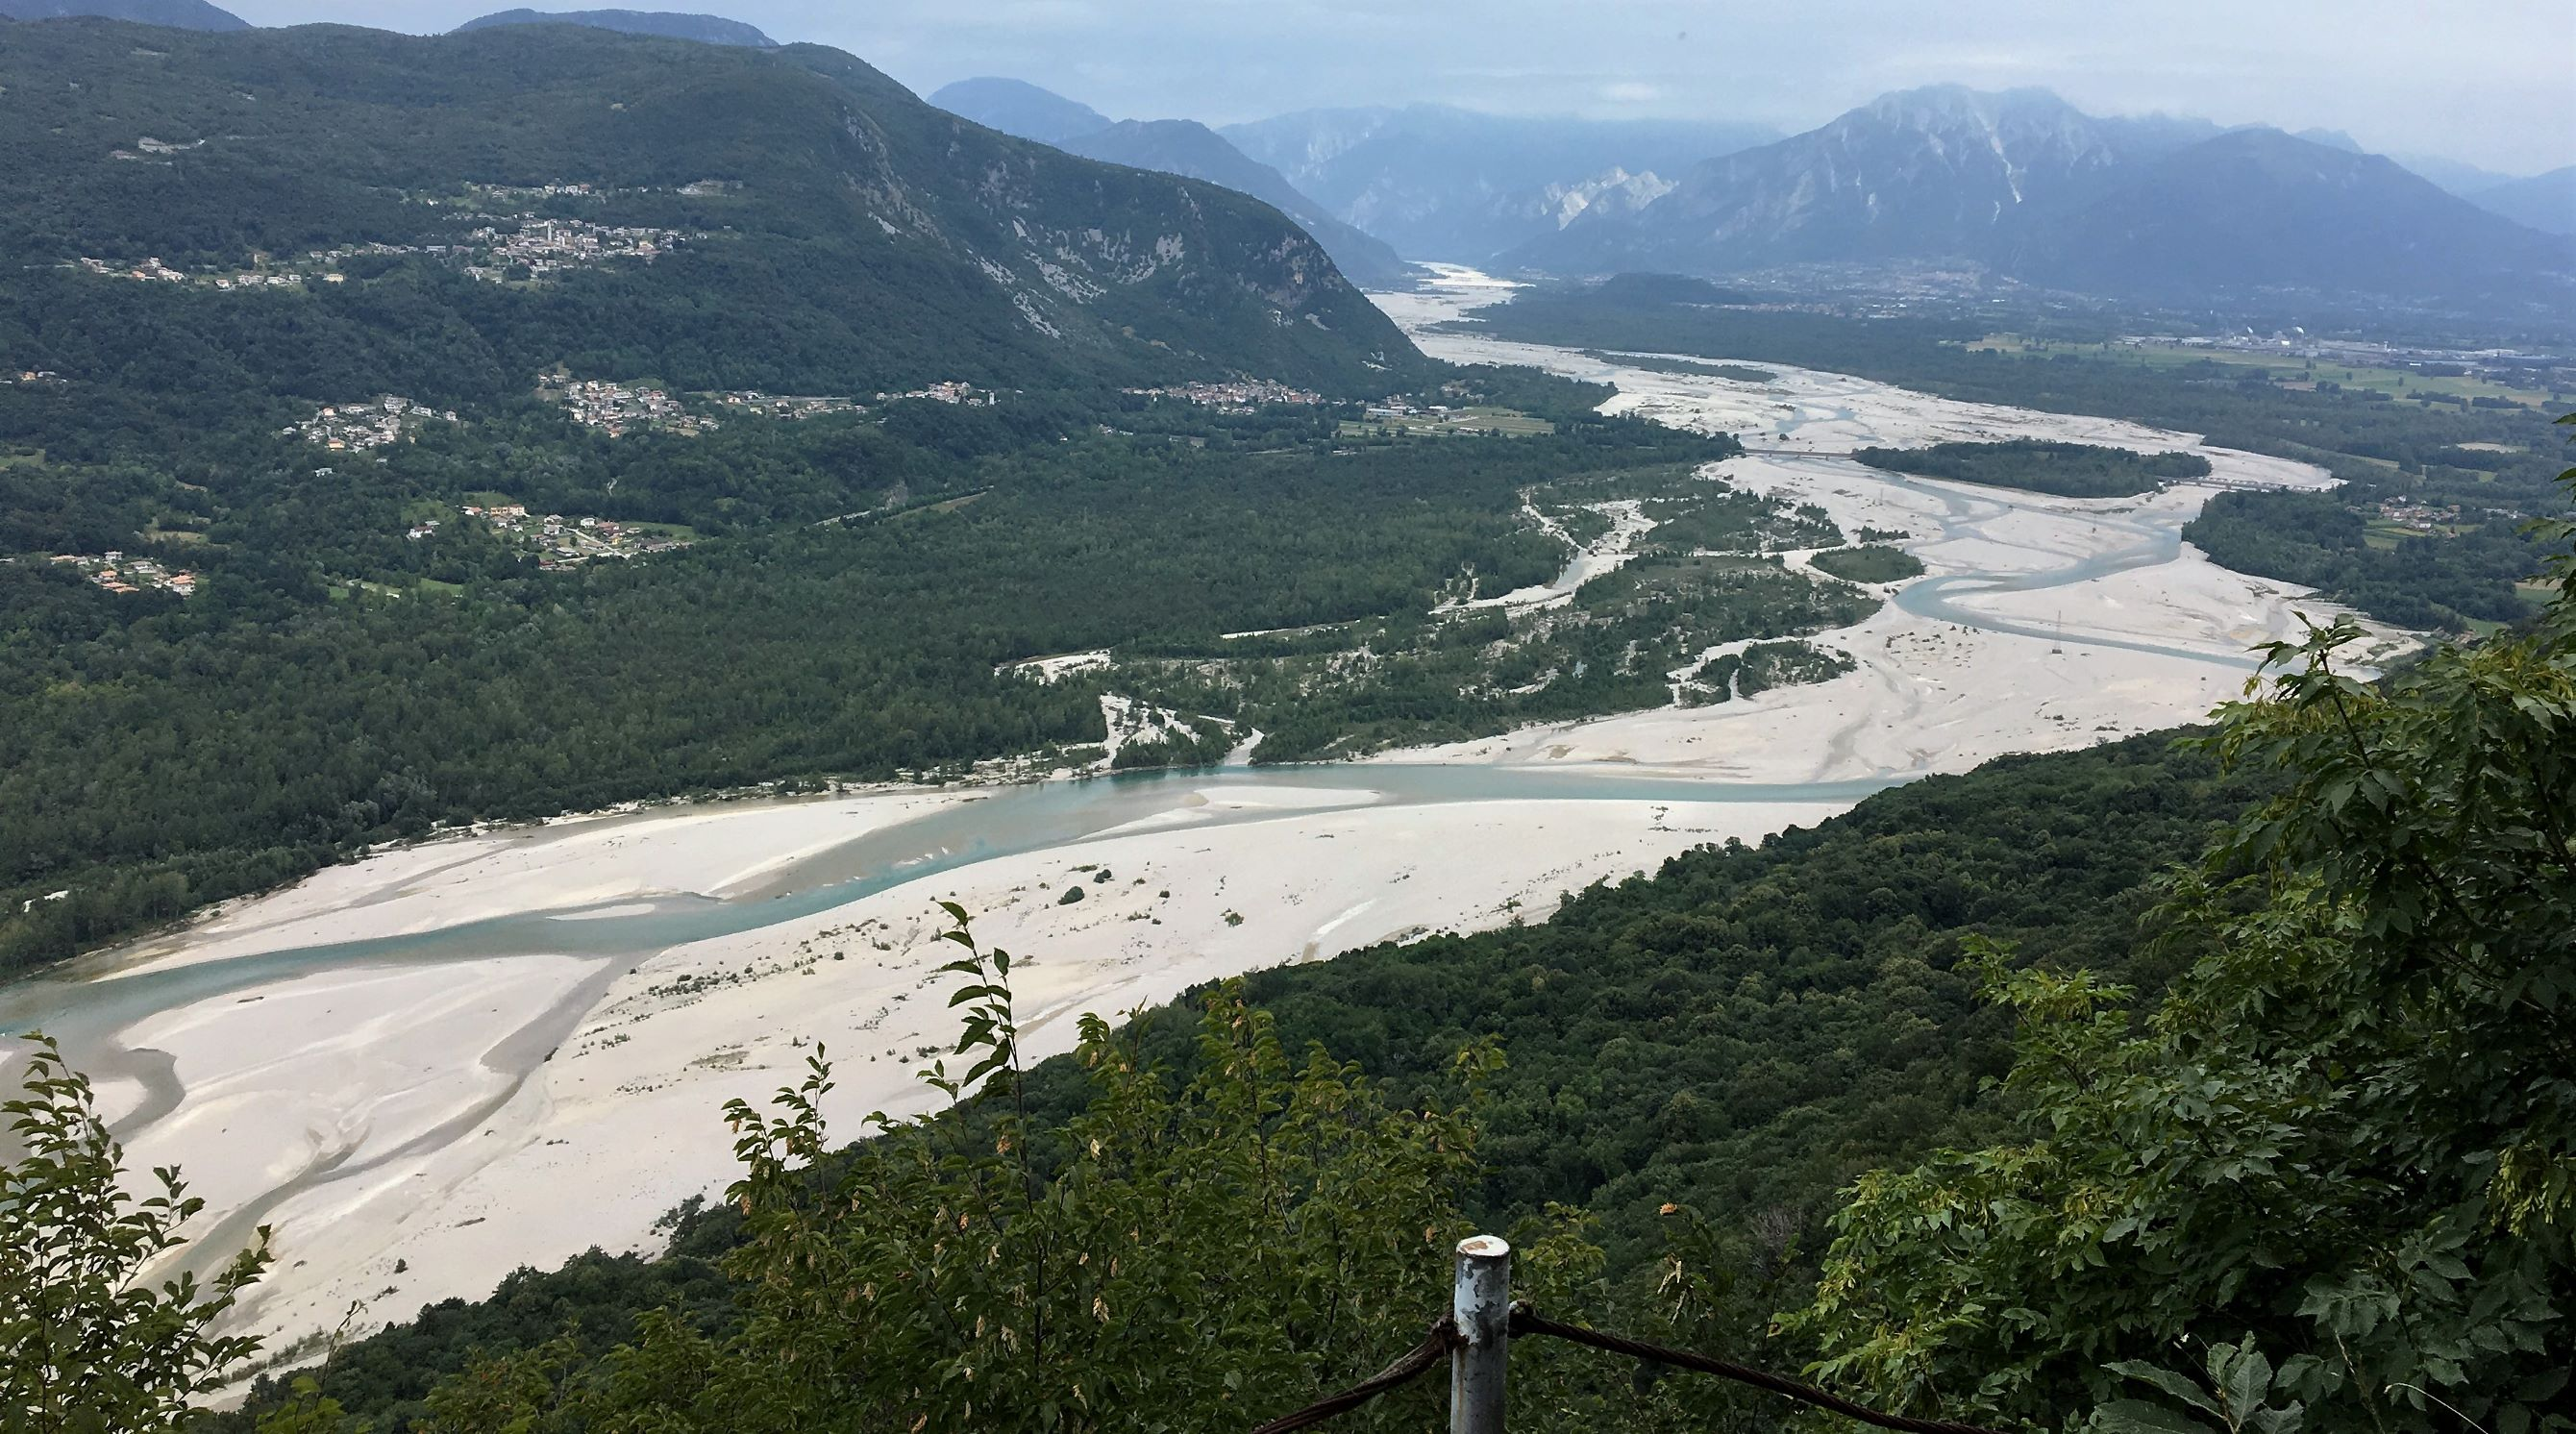
\includegraphics[width=\textwidth]{files/foto_flagogna.jpg}
	\caption[foto di un tratto del Tagliamento ripreso dal monte di Ragogna]{foto di un tratto del Tagliamento ripreso dal monte di Ragogna~(UD); l'acqua scorre da destra verso sinistra.
	}
	\label{fig:foto-ragogna}
\end{figure}



Questa prima figura mostra un fiume che scorre, libero, su un letto di ghiaia che forse pare essere decisamente più largo di quanto gli basterebbe. 
Dove sono gli argini? Il fiume può spostarsi? 
%
In mezzo alla figura si vedono numerose isole divise dal resto della vegetazione da canali abbandonati in ghiaia e sabbia. 
Come si formano? Rimangono inalterate al passare degli anni? 
%
Poco più in basso, dall'altra parte del canale, si intravedono degli arbusti proprio sulla ghiaia. 
Cresceranno fino a formare un'isola tanto vegetata quanto le vicine sue sorelle più a monte? O saranno spazzati via durante la prossima piena?

\medskip
Queste e altre cose si possono leggere da questa foto, così come da quella successiva. Tutte le domande hanno un carattere dinamico più o meno evidente: la loro risposta non la si può ottenere osservando una foto, che è statica, ma una sequenza di istanti successivi quale può essere un filmato.
Come racconta un professore, occorre sincronizzare i nostri orologi con quello del fiume; non solo, bisogna anche che indossiamo gli occhiali giusti per guardare i fenomeni alla scala in cui si possono vedere. Chi mai trarrebbe conclusioni effettive sulla vita di un albero se guardasse solo la sua foglia per pochi secondi, o se lo confrontasse su due immagini satellitari acquisite a distanza di diversi decenni?

\begin{figure}
	\centering
	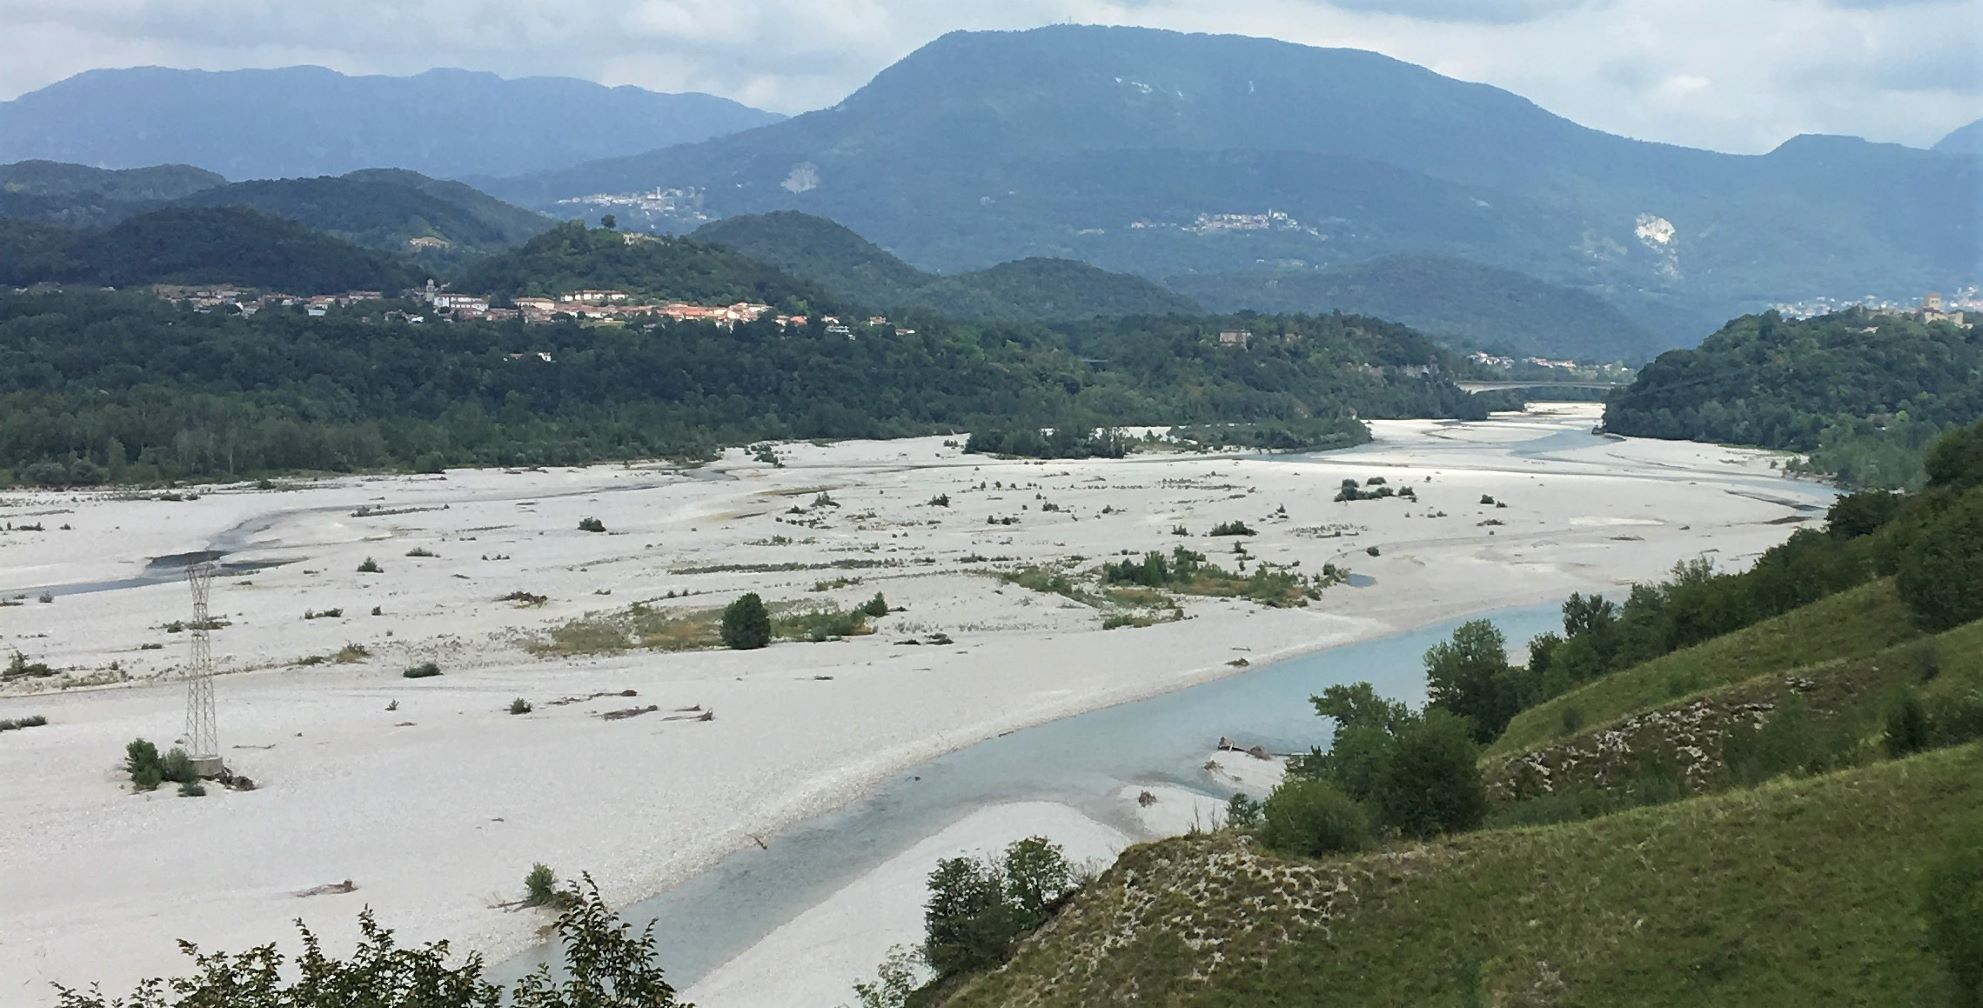
\includegraphics[width=\textwidth]{files/foto_terrazzo_valle_pinzano.jpg}
	\caption[foto di un tratto del Tagliamento ripreso dal terrazzo presso Aonedis~(UD)]{foto di un tratto del Tagliamento ripreso dal terrazzo presso Aonedis~(UD); l'acqua scorre da destra verso sinistra. 
	}
	\label{fig:foto-pinzano}
\end{figure}


Tra tutti i fiumi che ci sono nel nostro bel Paese, pochi di loro sono rimasti in condizioni “naturali”; l'alterazione ha apportato modifiche o ridotto l'entità dei processi che avevano luogo prima dell'intervento dell'uomo. 
Ad esempio, la costruzione di una diga a monte di un fiume può aver indotto nel corso degli anni un restringimento del suo alveo e ad un cambiamento della sua morfologia.
Ma in questo caso siamo fortunati: il Tagliamento può essere considerato un fiume alpino allo stato praticamente naturale.

Le domande che ho posto all'inizio nascono dalla curiosità che si può avere quando, dopo mesi di studio dei fenomeni che naturalmente avvengono nei fiumi, si incontra un fiume dove questi fenomeni possono accadere per davvero. Le domande trovano una risposta reale, comprovata da ciò che si vede quando si cammina sulla ghiaia, in mezzo alle isole, nei canali, e quando ci si tuffa nelle loro confluenze.

\medskip
La \cref{fig:confronto-imm-prefaz} mostra diversi processi che avvengono in questo fiume; questi, inutile ripeterlo, diventano apprezzabili solo dopo aver indossato gli occhiali e l'orologio giusti, cioè osservando da un'altezza di poche centinaia di metri da terra e confrontando immagini distanti pochi mesi. Ecco un'anteprima:
\begin{itemize}
	\item si vede subito che i canali migrano e si spostano durante gli anni; 
		difatti durante le piene più importanti tutto l'alveo si riempie di acqua e il fondo viene rimodellato;
	\item lo spostamento dei canali porta questi ad erodere lateralmente le isole, come si vede per l'isola in alto a sinistra in alveo; 
		il fiume quindi potrà trasportare non solo il materiale presente sul fondo, ma anche quello che erode dalle isole, sia ghiaia e sabbia che alberi;
	\item le isole possono espandersi da piccoli nuclei fino a unirsi, diventare più fitte e più resistenti all'erosione da parte dell'acqua, come si vede per la grande isola al centro della \cref{fig:confronto-imm-prefaz};
	\item l'erosione non risparmia le sponde, come si vede per la sponda a sinistra (in destra idrografica se si osserva il verso della corrente) la quale arretra di più di \SI{100}{\m} a causa delle piene che si susseguono nei tre anni di osservazione;
	\item l'erosione di isole e sponda produce moltissimo materiale legnoso (alberi sradicati) il quale si deposita poco più a valle della zona di erosione, come testimoniano i numerosi puntini scuri presenti sull'alveo asciutto; 
		se le condizioni sono adatte e se le piante sono in grado, è possibile che dai tronchi depositati crescano nuovi rami e radici; 
		questi tronchi diventano i nuclei di formazione di future isole;
	\item lo spostamento dei canali è limitato dalla presenza delle isole, che si configurano come ostacolo per la corrente anche durante le piene;
		difatti è difficile che il canale si possa spostare dove c'è l'isola in alto a destra, a meno che non riesca ad eroderla.
\end{itemize}

\begin{figure}
	\centering
	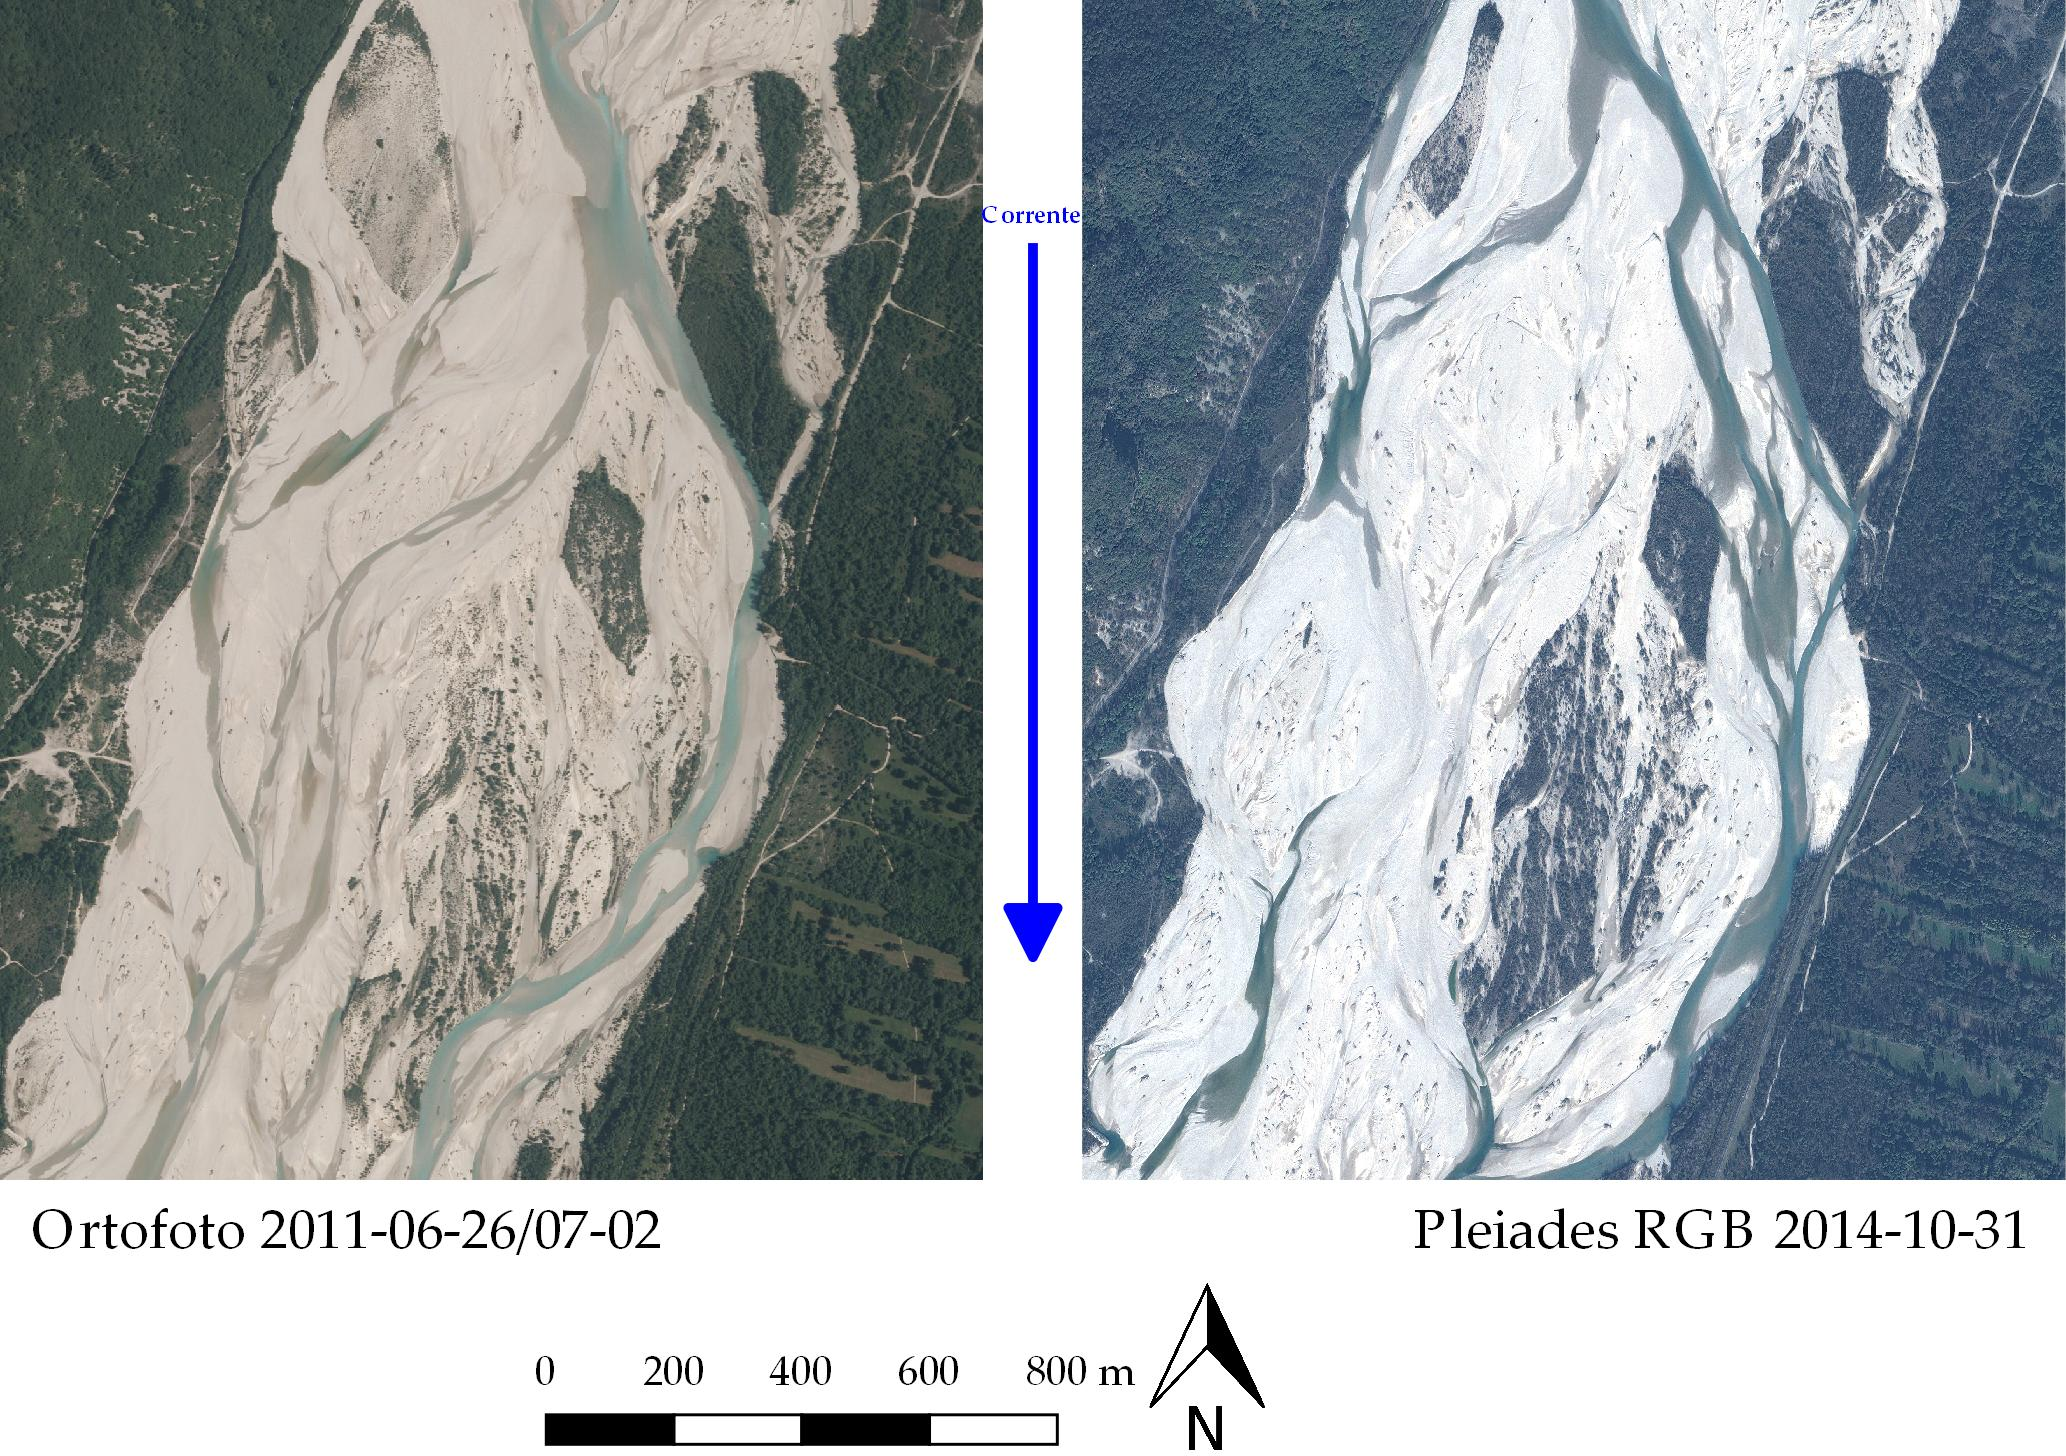
\includegraphics[width=\textwidth]{files/confronto_immagini_erosione_isole.jpeg}
	\caption[immagini di un tratto posto circa \SI{2}{\kilo\m} a monte del ponte di Cornino]{immagini di un tratto posto circa \SI{2}{\kilo\m} a monte del ponte di Cornino~(UD); l'ortofoto proviene dal Portale Cartografico Nazionale del Ministero dell'Ambiente.
	}
	\label{fig:confronto-imm-prefaz}
\end{figure}


Quante cose si possono osservare! In un fiume siffatto sono presenti numerosi altri fenomeni anche a scale diverse.
Ho raccontato quelli che mi interessano particolarmente e che sono oggetto di questa tesi: le dinamiche della vegetazione sulle isole e le dinamiche del legno depositato in alveo.

\medskip
A pensarci bene, non è sorprendente che in un sistema naturale la componente biologica influenzi fortemente quella fisica: i boschi consolidano i pendii e le foreste determinano la forma meandriforme di molti fiumi. Attraverso altri esempi ci si può convincere che le isole vegetate e i tronchi che rigettano in arbusti possano esercitare effetti su un fiume e viceversa. 
\\
E riflettendo ancora non è difficile osservare che queste interazioni solitamente possono indurre effetti positivi sia per l'ambiente che per l'essere umano: per portare qualche esempio, nel caso del Tagliamento si parla di biodiversità data da un mosaico in continuo cambiamento di ambienti diversi, di purificazione dell'acqua, del mantenimento di un microclima particolarmente adatto alla stagionatura del prosciutto di San Daniele (prodotto nell'omonimo paese poco distante) e di un luogo molto adatto per la ricreazione da parte delle persone (\cref{fig:bagnanti}).

Da questi fatti muovo i primi passi verso l'approfondimento dei processi che portano un fiume a modificarsi di continuo assieme all'ambiente in cui si colloca.


\begin{figure}[hb]
	\centering
	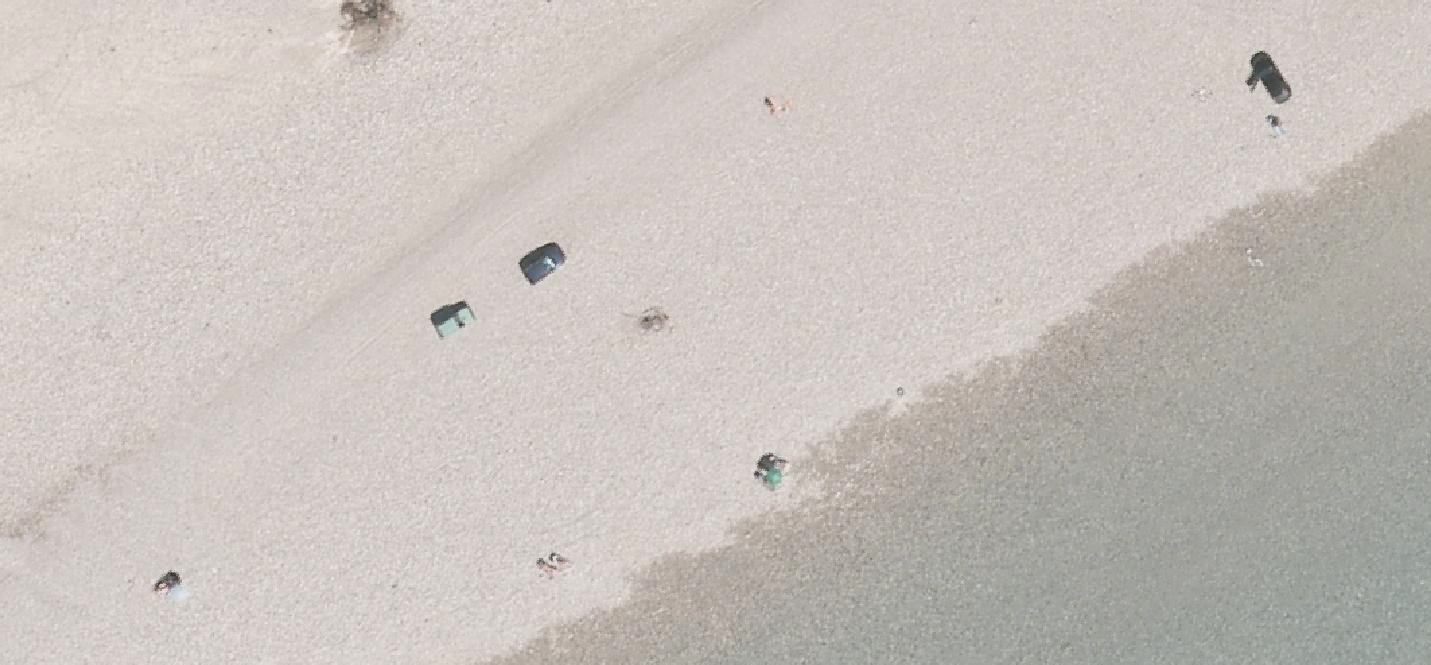
\includegraphics[width=\textwidth]{files/bagnanti.jpeg}
	\caption[bagnanti accanto ad un canale]{bagnanti accanto ad un canale ripresi con una immagine area del~2011, cortesemente fornita da Nicola Surian (Università degli studi di Padova).}
	\label{fig:bagnanti}
\end{figure}



%----------------------------------------------------------



%**********************************************************
%**********************************************************
\mainmatter
\chapter{Inizio}
\section{Introduzione}
La presente tesi mira a studiare come cambia la vegetazione nel fiume Tagliamento in risposta al regime idrologico (successione di magre, piene bankfull, flood pulses). 
L'obiettivo principale è quello di ricercare una relazione tra i livelli del pelo libero registrati da un idrometro e la quantità di vegetazione presente in alveo, tra i livelli e la quantità di legname che si ritrova in alveo dopo eventi di piena.

Si analizzano immagini satellitari e ortofoto al fine di distinguere la parte dell'alveo ricoperta da vegetazione (\vref{fig:esempio-isola-1}) e gli elementi legnosi (tronchi e accumuli di legno, \vref{fig:esempio-accumulo-1}).

\begin{figure}
	\centering
	\begin{subfigure}[b]{0.37\textwidth}
		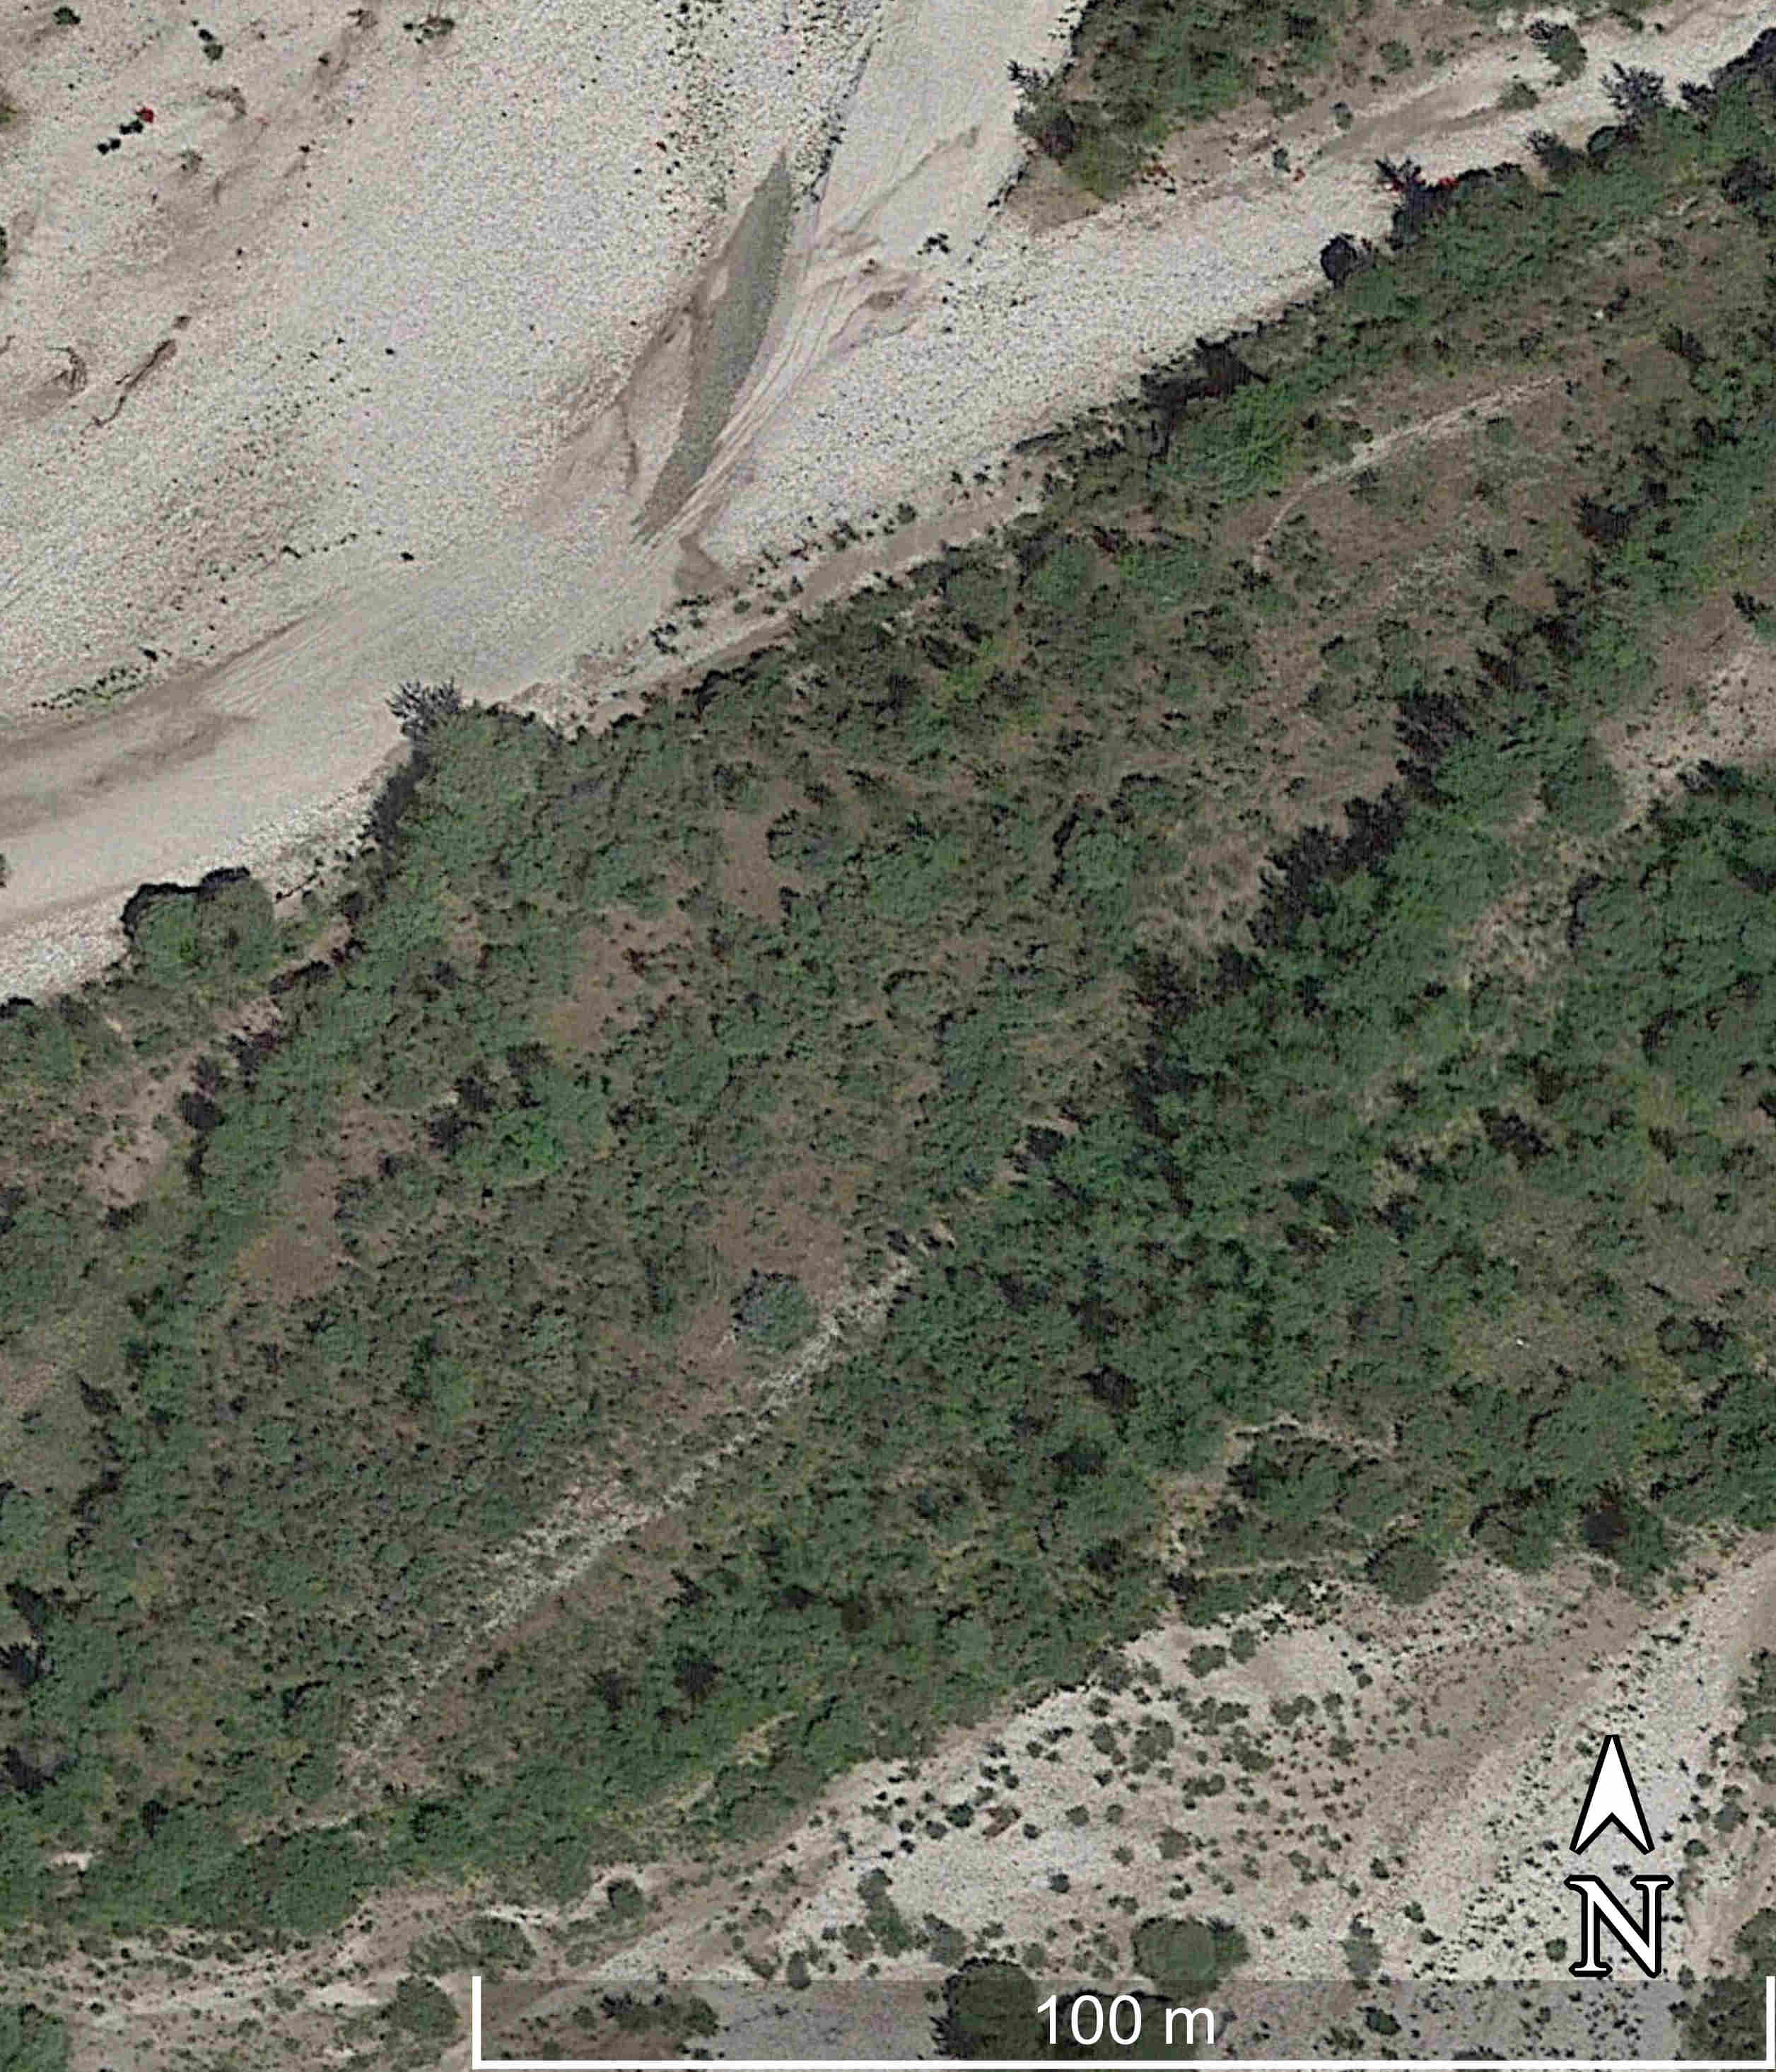
\includegraphics[width=\textwidth]{files/esempio_isola_sat_1.jpg}
		\caption{immagine da Google Earth di un isola in alveo.}
		\label{fig:esempio-isola-sat-1}
	\end{subfigure}
	\quad
	\begin{subfigure}[b]{0.57\textwidth}
		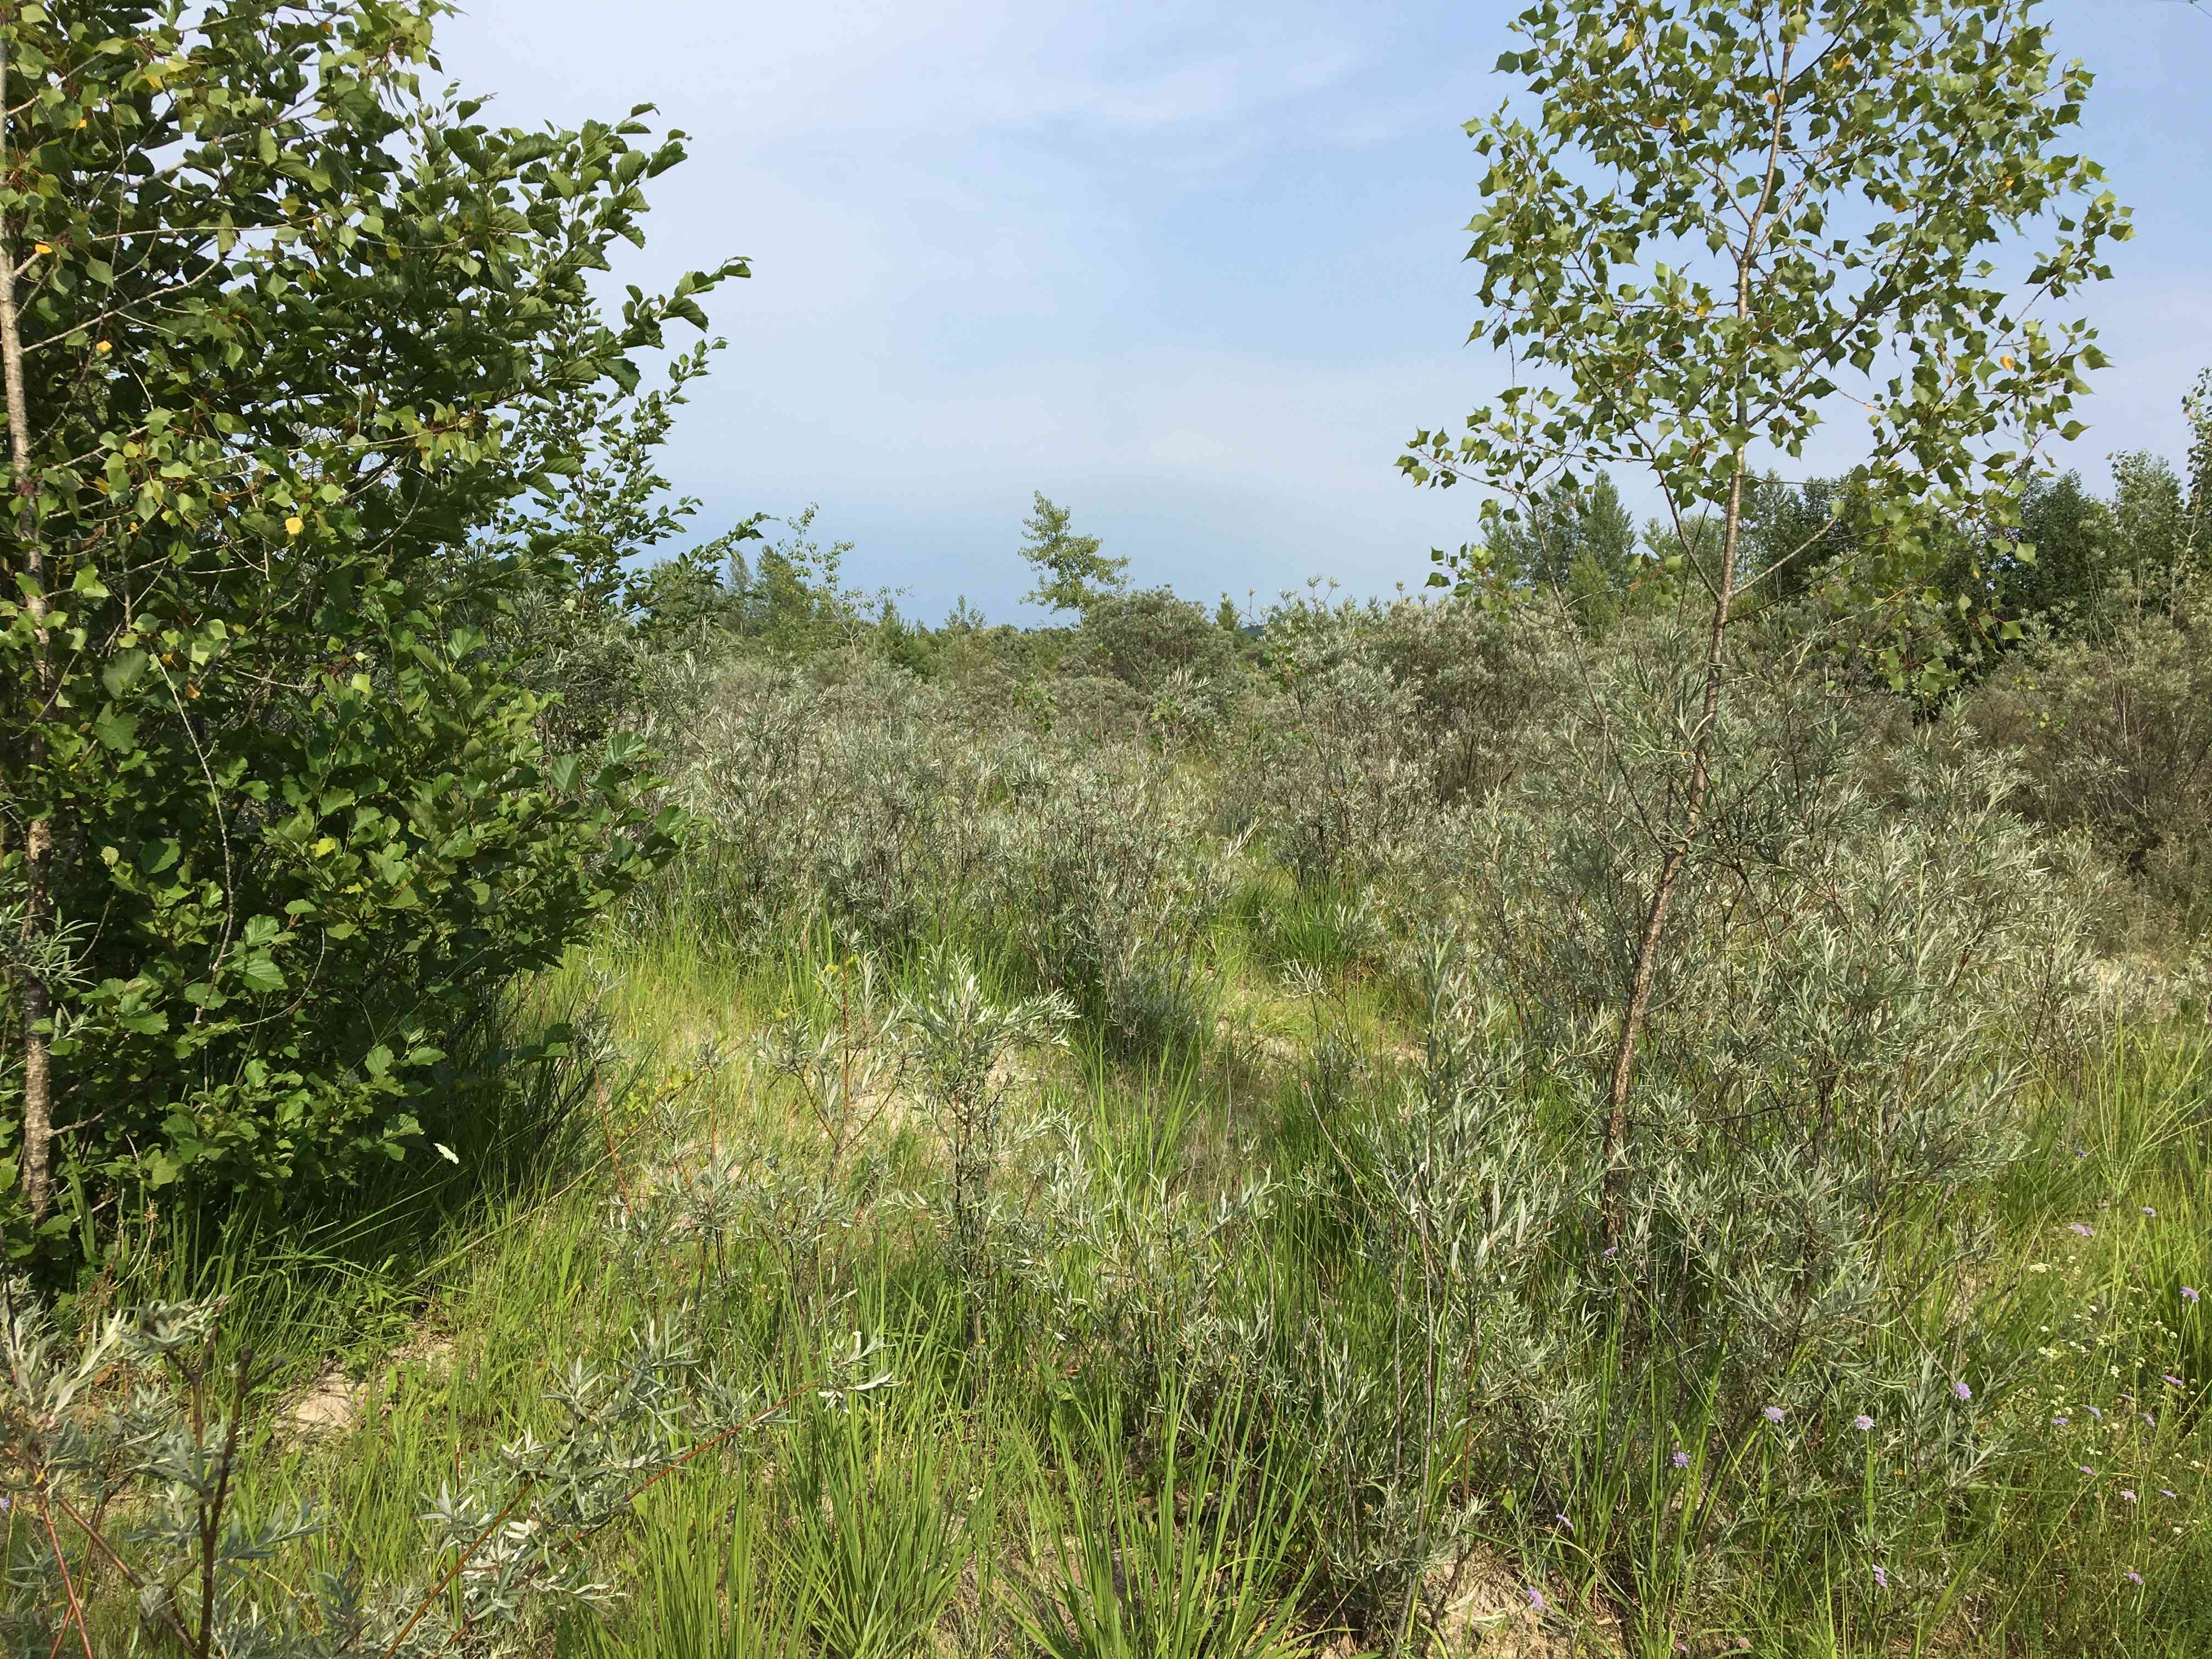
\includegraphics[width=\textwidth]{files/esempio_isola_1.jpg}
		\caption{foto di un isola molto vegetata presente nell'alveo del fiume.
		Foto dell'autore.}
		\label{fig:esempio-isola-1}
	\end{subfigure}
	\caption[immagine e foto di isole fluviali]{immagine e foto di isole fluviali; si noti la forte presenza di salici (\emph{Salix spp.}) e di pioppi (\emph{Populus spp.}); il luogo della foto è prossimo a quello dell'immagine.}
\end{figure}

\begin{figure}
	\centering
	\begin{subfigure}[b]{0.52\textwidth}
		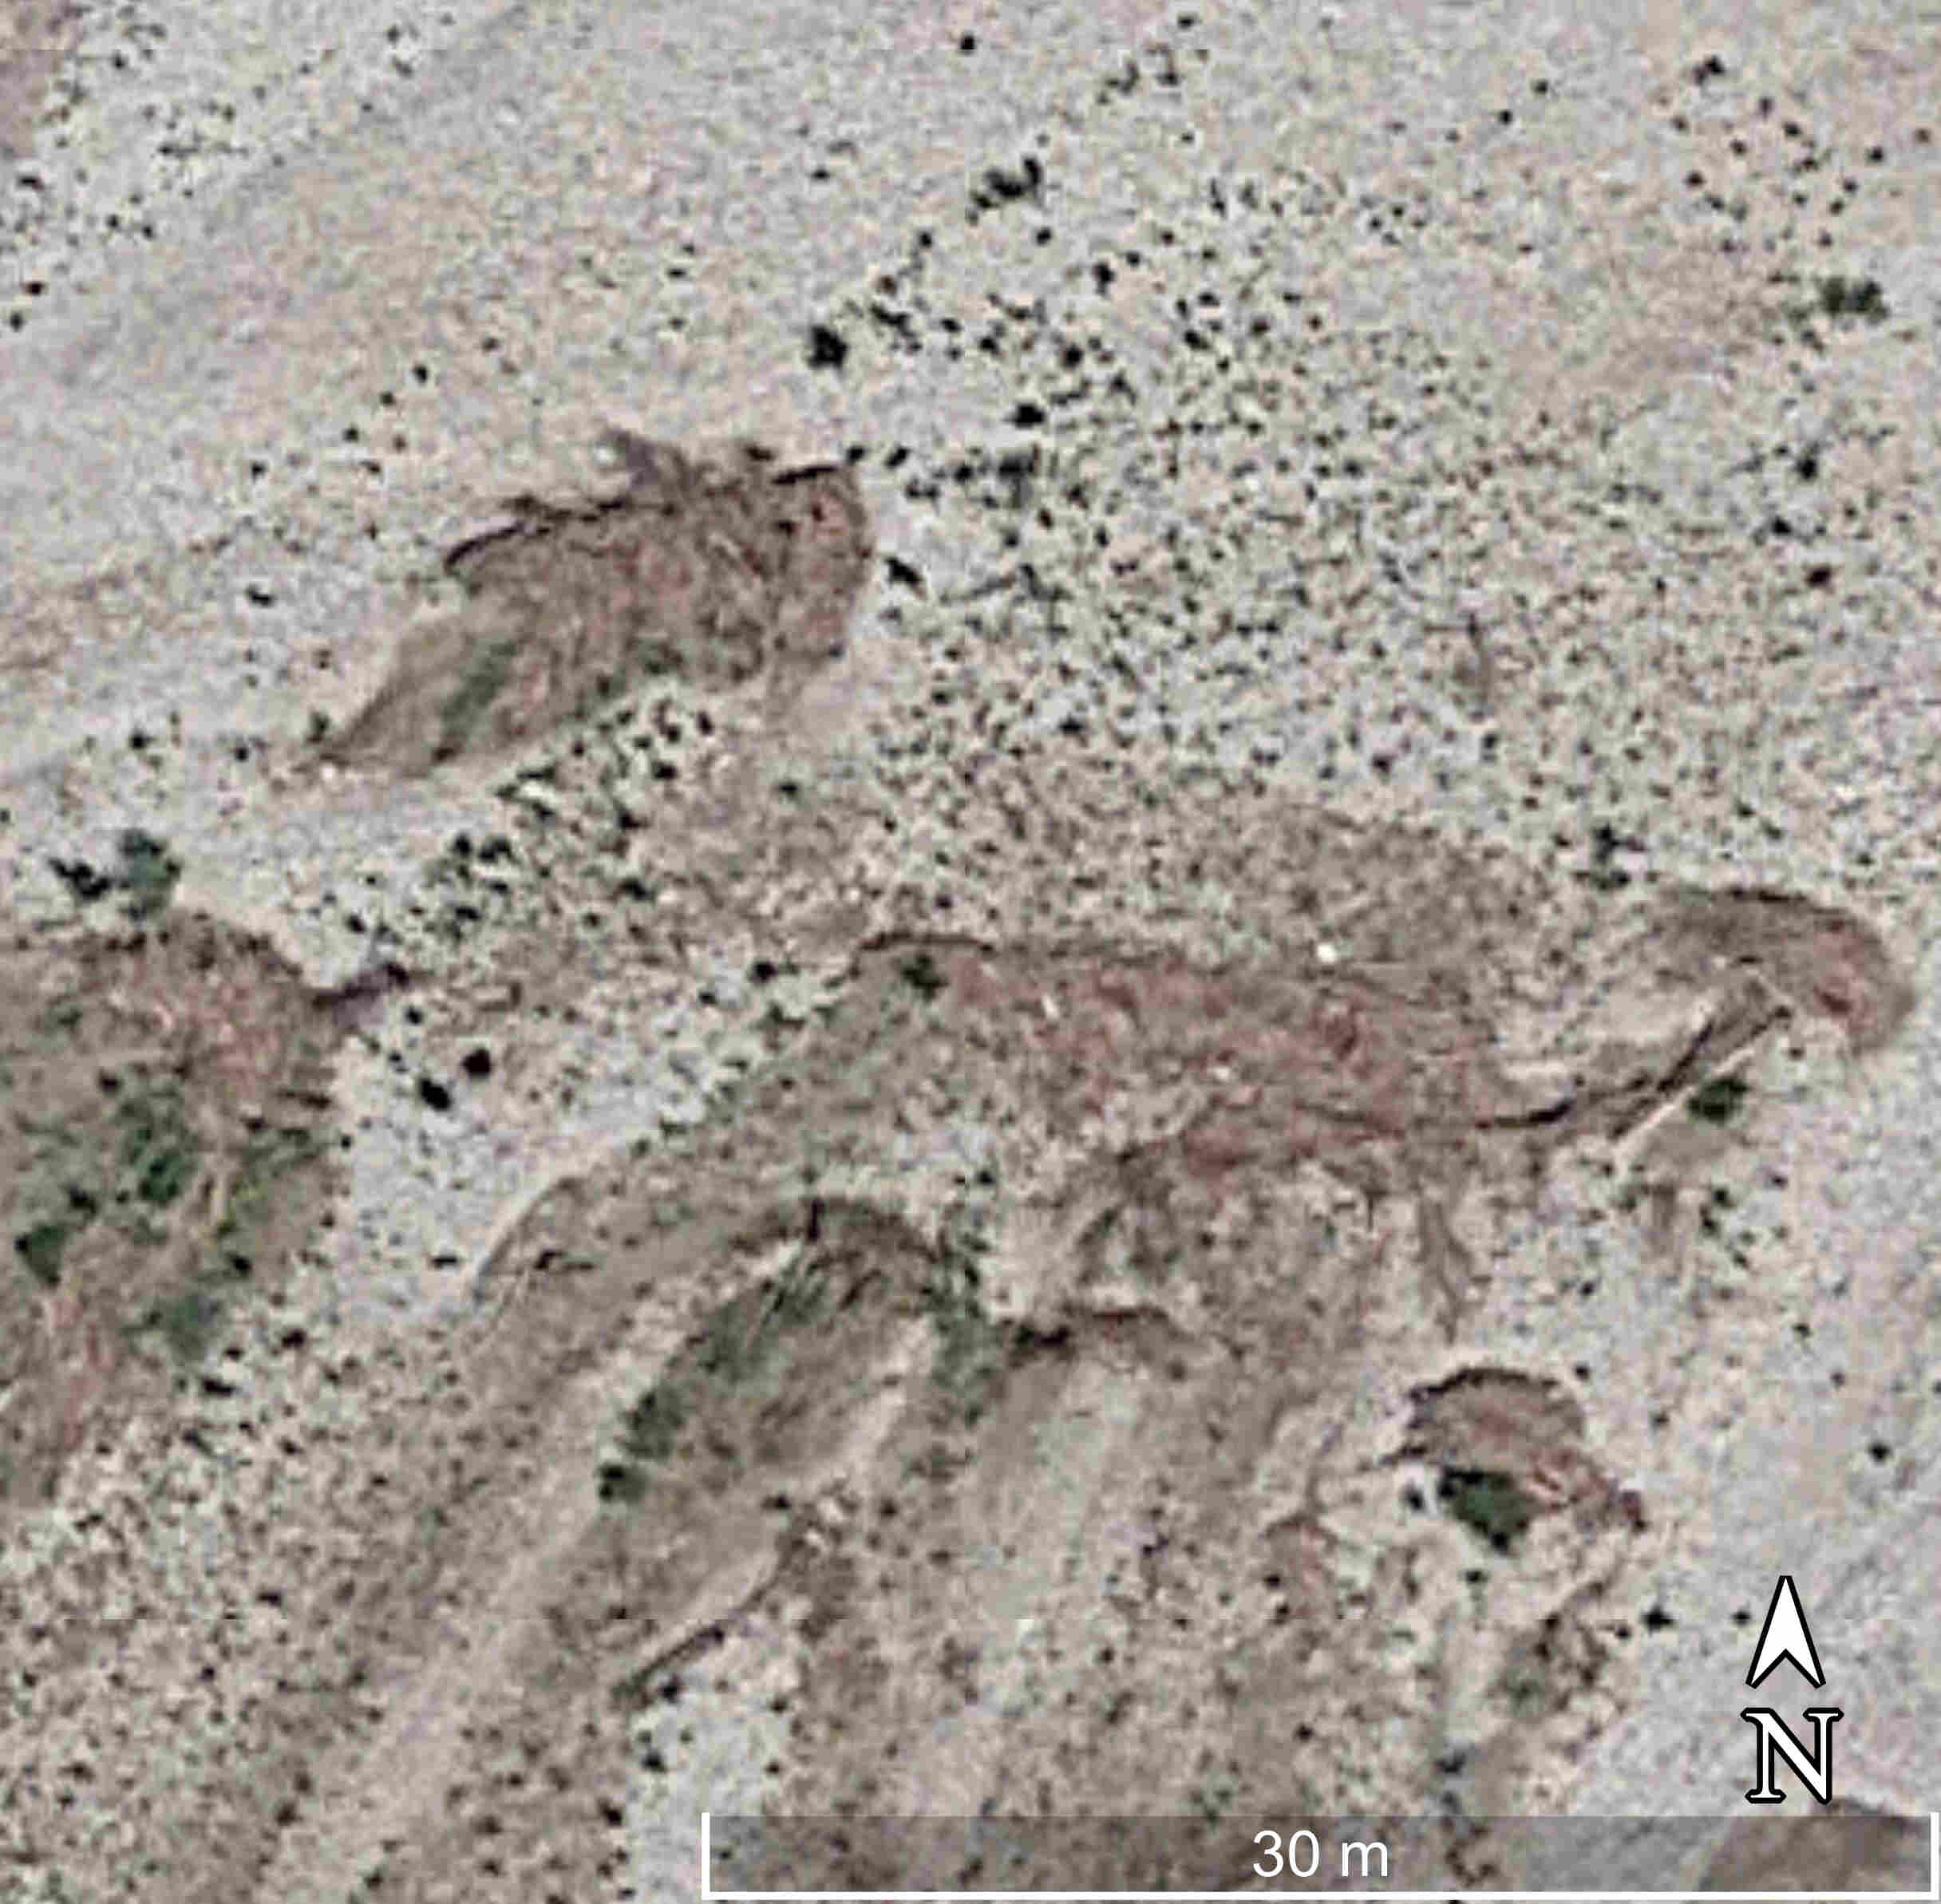
\includegraphics[width=\textwidth]{files/esempio_accumulo_sat_1.jpg}
		\caption{immagine da Google Earth di accumuli di legno e tronchi in alveo (in marrone chiaro).}
		\label{fig:esempio-accumulo-sat-1}
	\end{subfigure}
	\quad
	\begin{subfigure}[b]{0.44\textwidth}
		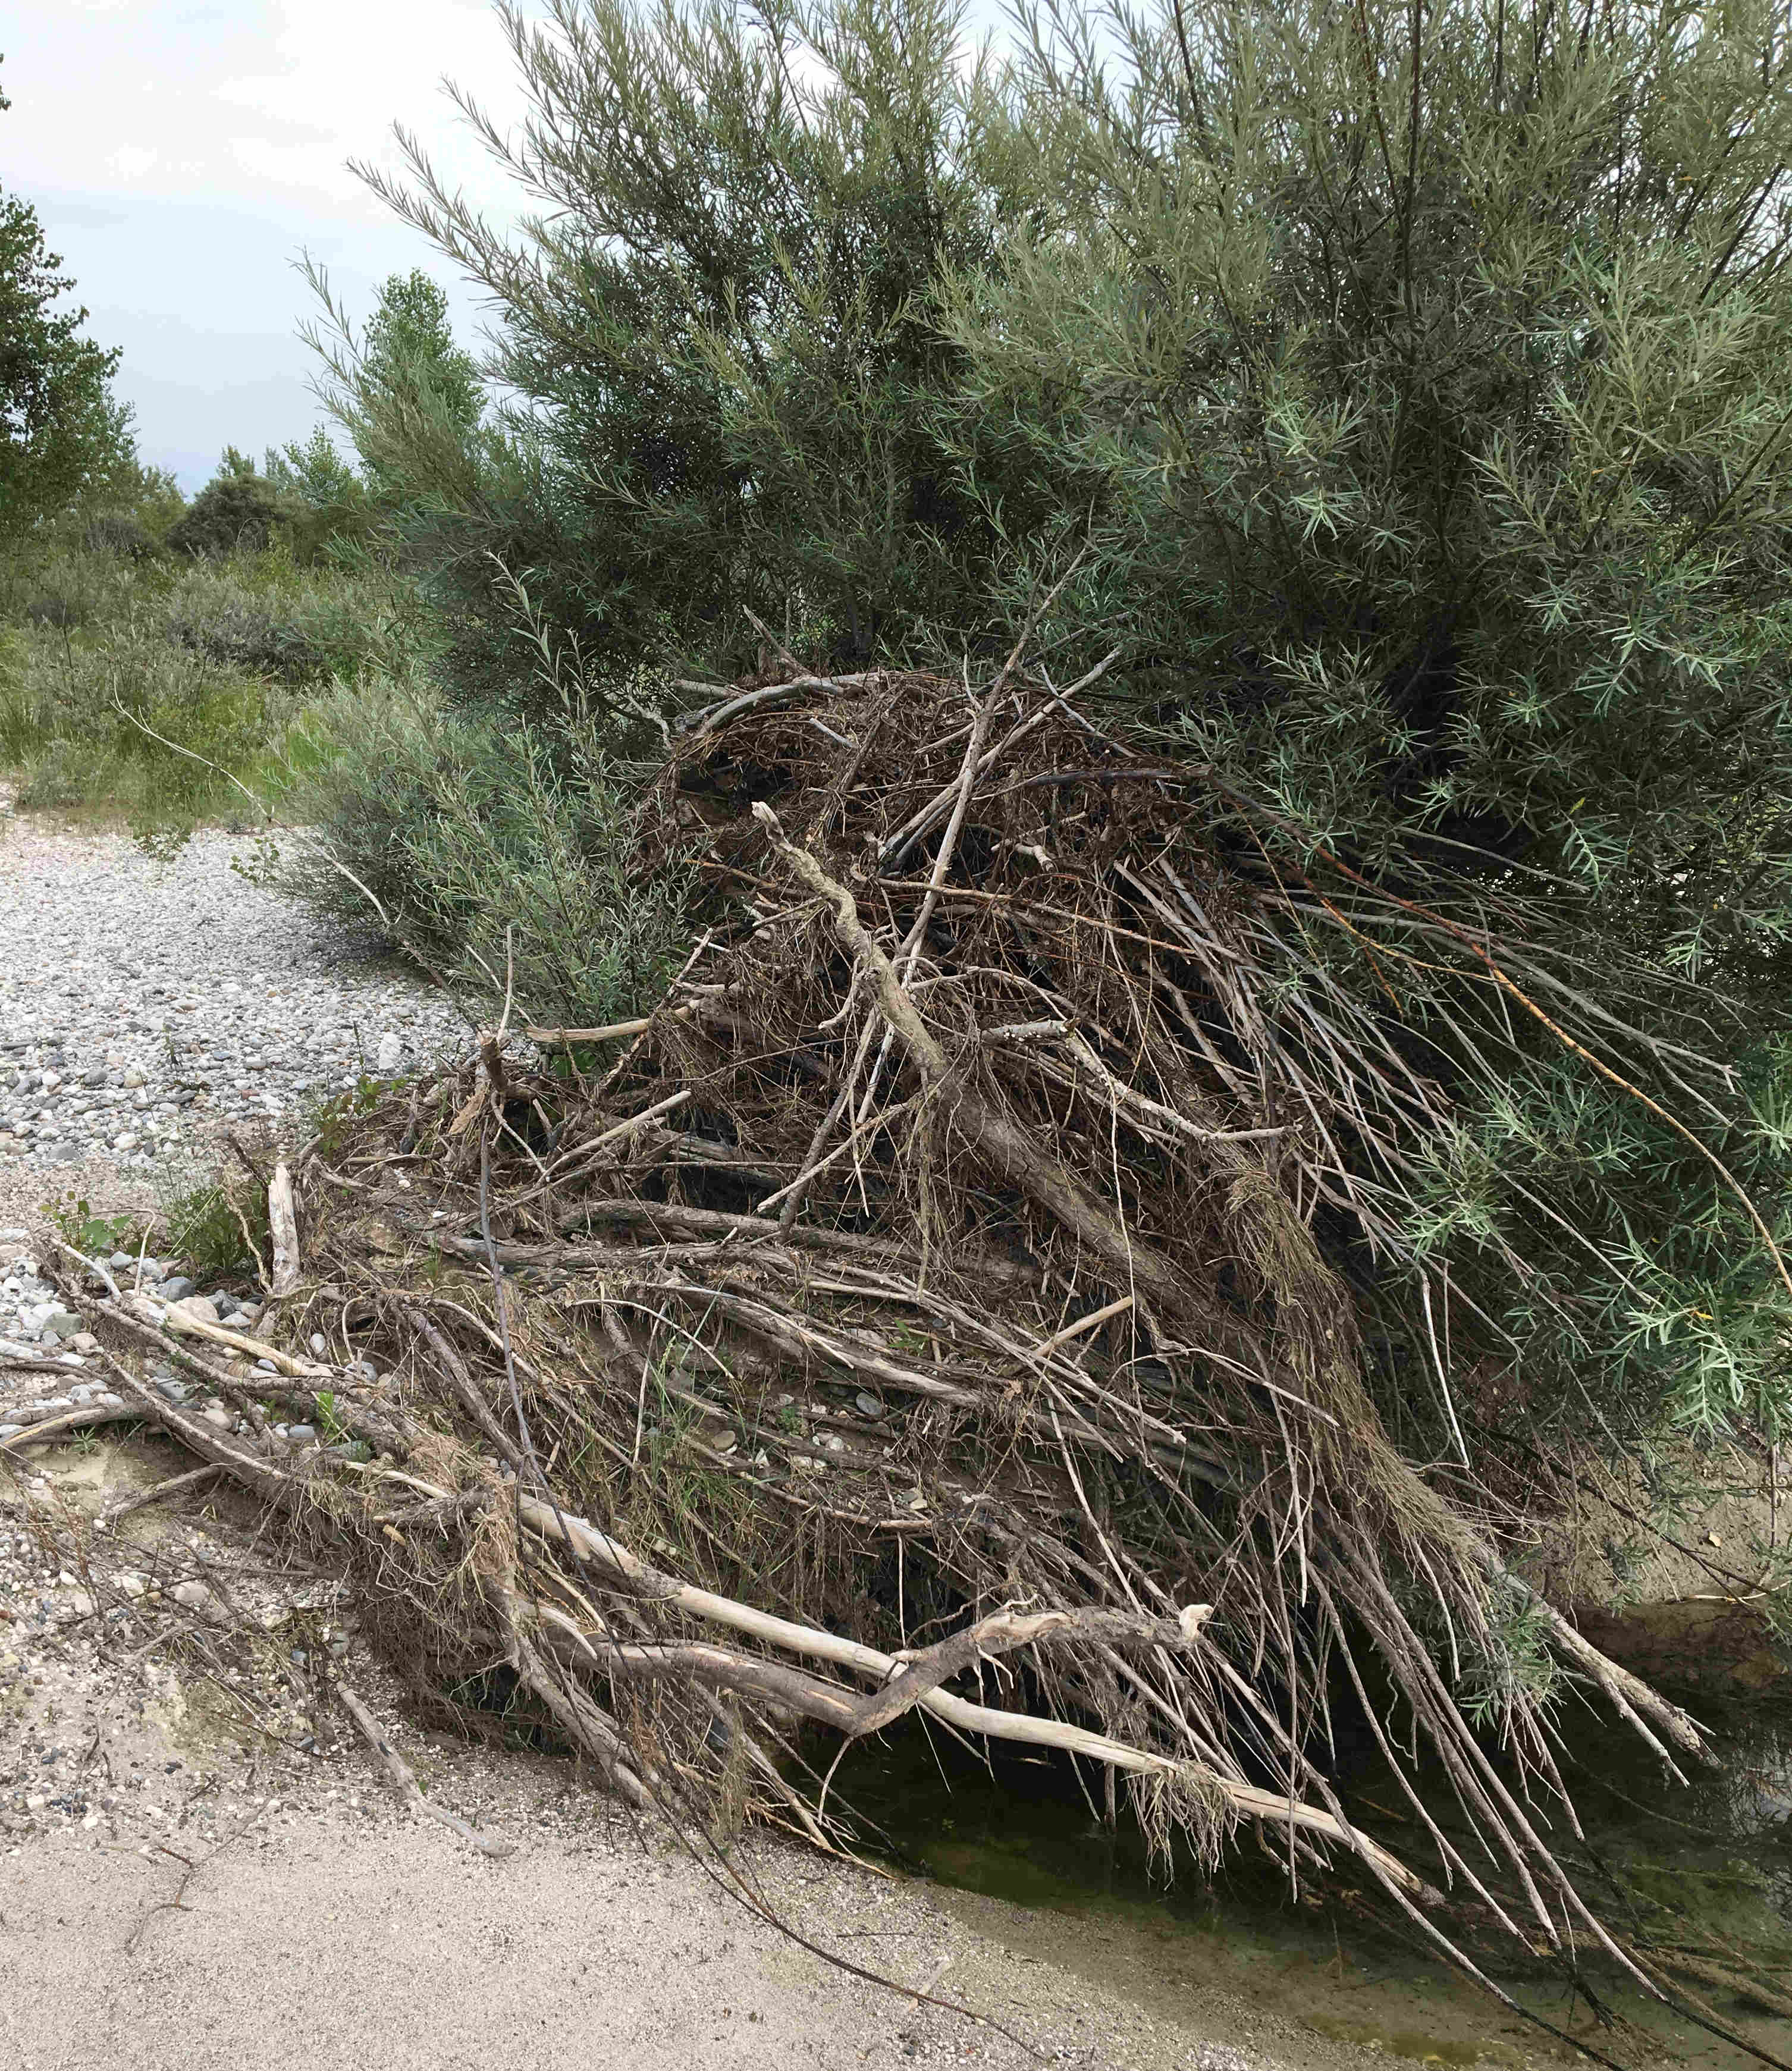
\includegraphics[width=\textwidth]{files/esempio_accumulo_1.jpg}
		\caption{foto di un accumulo di tronchi sopra una pianta di salice.
		Foto dell'autore.}
		\label{fig:esempio-accumulo-1}
	\end{subfigure}
	\caption[immagine e foto di accumuli legnosi]{immagine e foto di accumuli legnosi. Il luogo della foto non corrisponde a quello dell'immagine.}
\end{figure}

Con i dati di piovosità media mensile e di temperatura media mensile si cercano correlazioni con l'espansione della vegetazione che si osserva negli anni.
Dalla quantificazione dell'erosione della vegetazione dovuta alle piene, della quantità di legno in alveo e di un tasso di crescita della vegetazione si tenta di costruire un bilancio di materia vegetale a scala di evento di piena.
Inoltre si trovano valori soglia del livello del pelo libero per l'erosione della vegetazione.


\section{Bande spettrali}
Gli strumenti di acquisizione di immagini aeree e satellitari sono sensibili a determinate bande della radiazione elettromagnetica (\vref{graph:el-mag-radiation}), cioè sono in grado di registrarne solo alcune porzioni. 
L'occhio umano può distinguere solo le bande del visibile, mentre i sensori artificiali possono acquisire altre bande della radiazione. 
%
\begin{figure}
	\centering
	\tikzsetnextfilename{electromagnetic_radiation}
\begin{tikzpicture}[fill between/on layer={axis grid}]
	\begin{axis}[
		xlabel={Lunghezza d'onda},
		xticklabel style = {font=\tiny,yshift=0.2ex},
		xmin=10^-5,
		xmax=10^9,
		x unit=\si{\micro\meter},
		xmode=log,
		ymin=0,
		ymax=1,
		height=3cm,
		width=\textwidth,%12.2cm,
		yticklabels={},
		ytick=\empty,
		legend cell align=left,
		legend style={
			at={(0.5,-0.8)},%(0.85,-0.77)},
			anchor=north,
			legend columns=4,
			}
	]
	\addplot[draw=none, name path=start, forget plot] coordinates{(10^-5,0)(10^-5,1)};
	\addplot[draw=none, name path=gamma, forget plot] coordinates{(10^-3,0)(10^-3,1)};
	\addplot[draw=none, name path=xrays, forget plot] coordinates{(10^-2,0)(10^-2,1)};
	\addplot[draw=none, name path=uv, forget plot] coordinates{(0.4,0)(0.4,1)};
	\addplot[draw=none, name path=visible, forget plot] coordinates{(0.7,0)(0.7,1)};
	\addplot[draw=none, name path=ir, forget plot] coordinates{(10^2.5,0)(10^2.5,1)};
	\addplot[draw=none, name path=microwave, forget plot] coordinates{(10^5,0)(10^5,1)};
	\addplot[draw=none, name path=radiowave, forget plot] coordinates{(10^9,0)(10^9,1)};
	\addplot[violet!20, area legend] fill between[of=start and gamma];
	\addlegendentry{Raggi $\gamma$}
	\addplot[violet!60, area legend] fill between[of=gamma and xrays];
	\addlegendentry{Raggi X}
	\addplot[violet, area legend] fill between[of=xrays and uv];
	\addlegendentry{Ultravioletti}
	\addplot[shading=visiblelight, area legend] fill between[of=uv and visible];
	\addlegendentry{Luce visibile}
	\addplot[red, area legend] fill between[of=visible and ir];
	\addlegendentry{Infrarosso}
	\addplot[Bittersweet, area legend] fill between[of=ir and microwave];
	\addlegendentry{Microonde}
	\addplot[Brown, area legend] fill between[of=microwave and radiowave];
	\addlegendentry{Onde radio}
	\end{axis}
\end{tikzpicture}

	\caption{radiazione elettromagnetica con le sue lunghezze d'onda.}
	\label{graph:el-mag-radiation}
\end{figure}
%
\\
Le immagini nel visibile sono solitamente suddivise nelle bande del Rosso, Verde e Blu (\emph{Red}, \emph{Green}, \emph{Blue}, RGB); ognuna indica la quantità di colore presente; la combinazione di queste quantità di colore restituisce l'immagine a colori. 
\\
Per poter osservare immagini con bande diverse dal visibile si sostituisce una o più bande RGB con le bande in questione. 
Ad esempio, è possibile sostituire la banda del Rosso con quella dell'Infrarosso (IR): la quantità di colore del Rosso sarà rimpiazzata dalla quantità di colore dell'Infrarosso. 
Il risultato sarà un'immagine riconoscibile dall'occhio umano, ma in falsi colori (\vref{fig:confronto-bande-intro}).
%
\begin{figure}
	\centering
	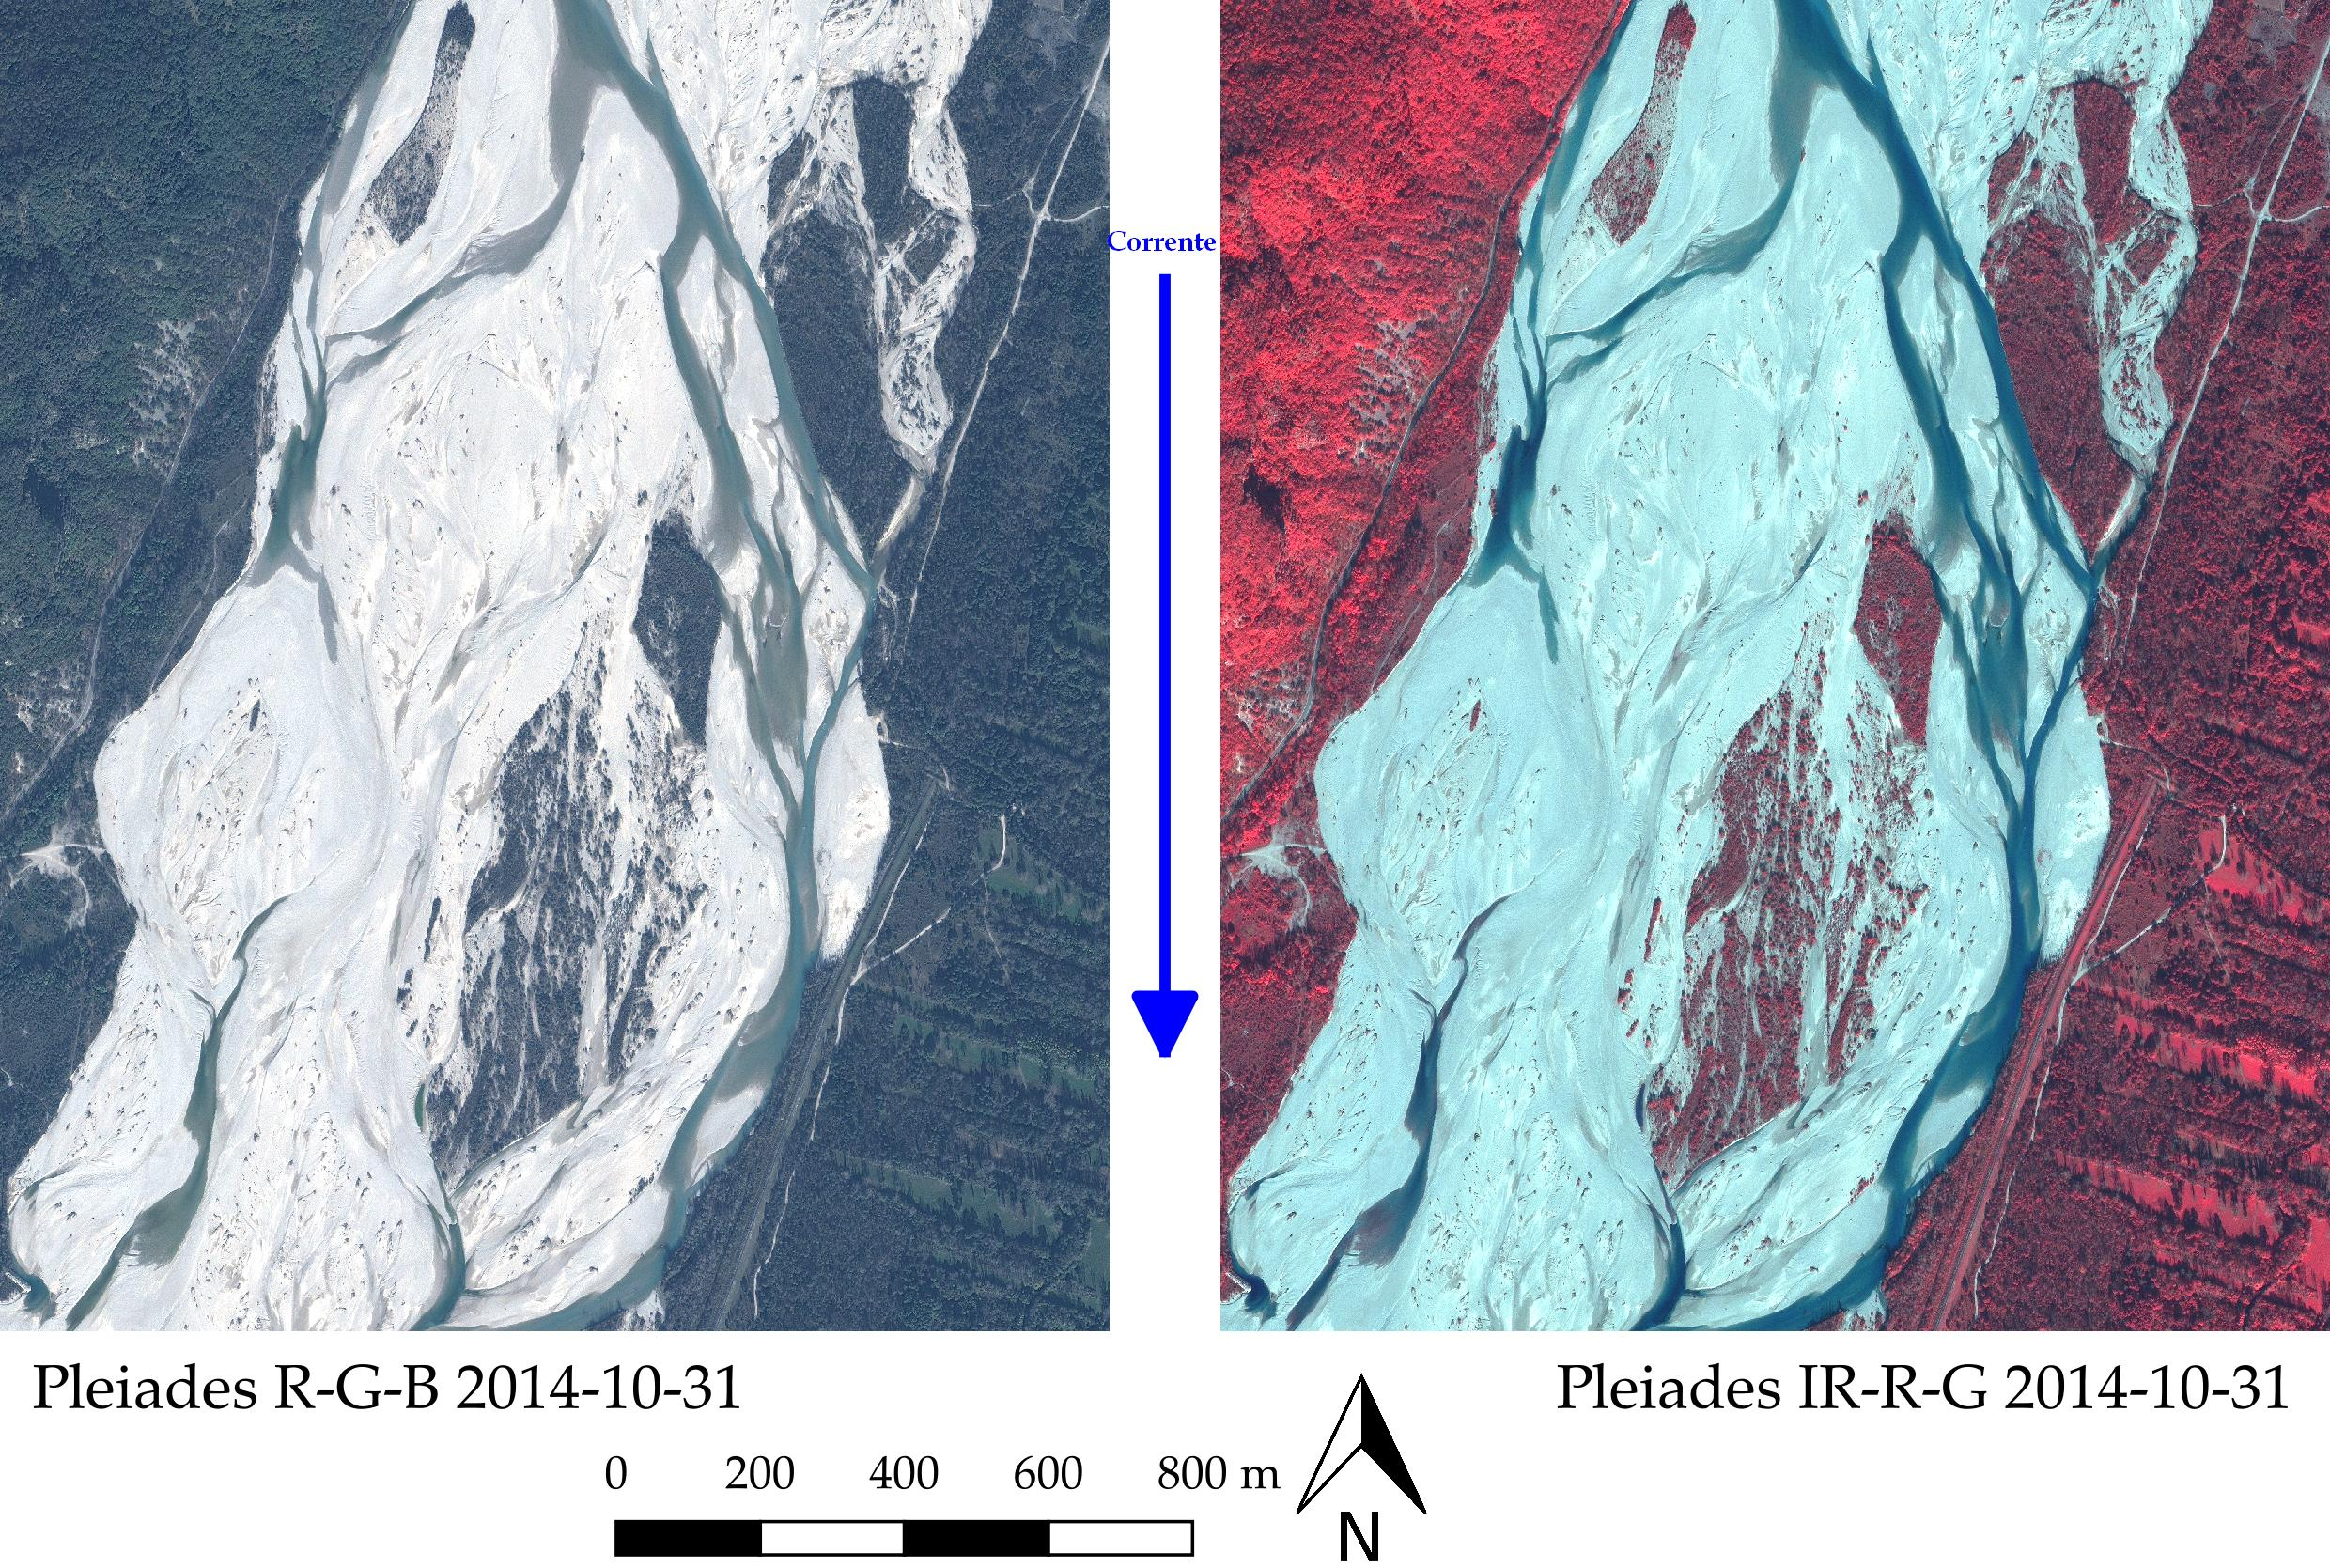
\includegraphics[width=\textwidth]{files/confronto_bande_intro.jpeg}
	\caption[confronto immagini R-G-B e IR-R-G]{confronto di un'immagine in veri colori (R-G-B, a sinistra) con una in falsi colori (IR-G-B, a destra); quest'ultima evidenza la presenza di vegetazione viva rispetto alla ghiaia in alveo e all'acqua nei canali.}
	\label{fig:confronto-bande-intro}
\end{figure} 
%
\\
Questo procedimento serve per distinguere più facilmente degli elementi e degli oggetti presenti nelle immagini; per esempio la vegetazione viva riflette particolarmente la banda dell'Infrarosso più vicina al Rosso.




\section{Inquadramento dell'area di studio}
Il Fiume Tagliamento, situato nel Nord-Est italiano, è uno dei pochi fiumi alpini allo stato quasi naturale. 
Il suo bacino idrografico, ampio circa~\SI{2900}{\kilo\m\tothe{2}}, si estende tra le province di Udine, Pordenone e Venezia.
Il suo corso di circa~\SI{170}{\kilo\m} presenta morfologia intrecciata (\emph{braided}) nelle parti montane e planiziali; verso valle il fiume si restringe assumendo prima una forma transizionale monocursale nei pressi di Madrisio, infine meandriforme a Latisana.
\\
Il tratto studiato è quello intrecciato multicanale compreso tra Tolmezzo e Madrisio (\vref{fig:overview,fig:overview-gearth}).
%
\begin{figure}
	\centering
	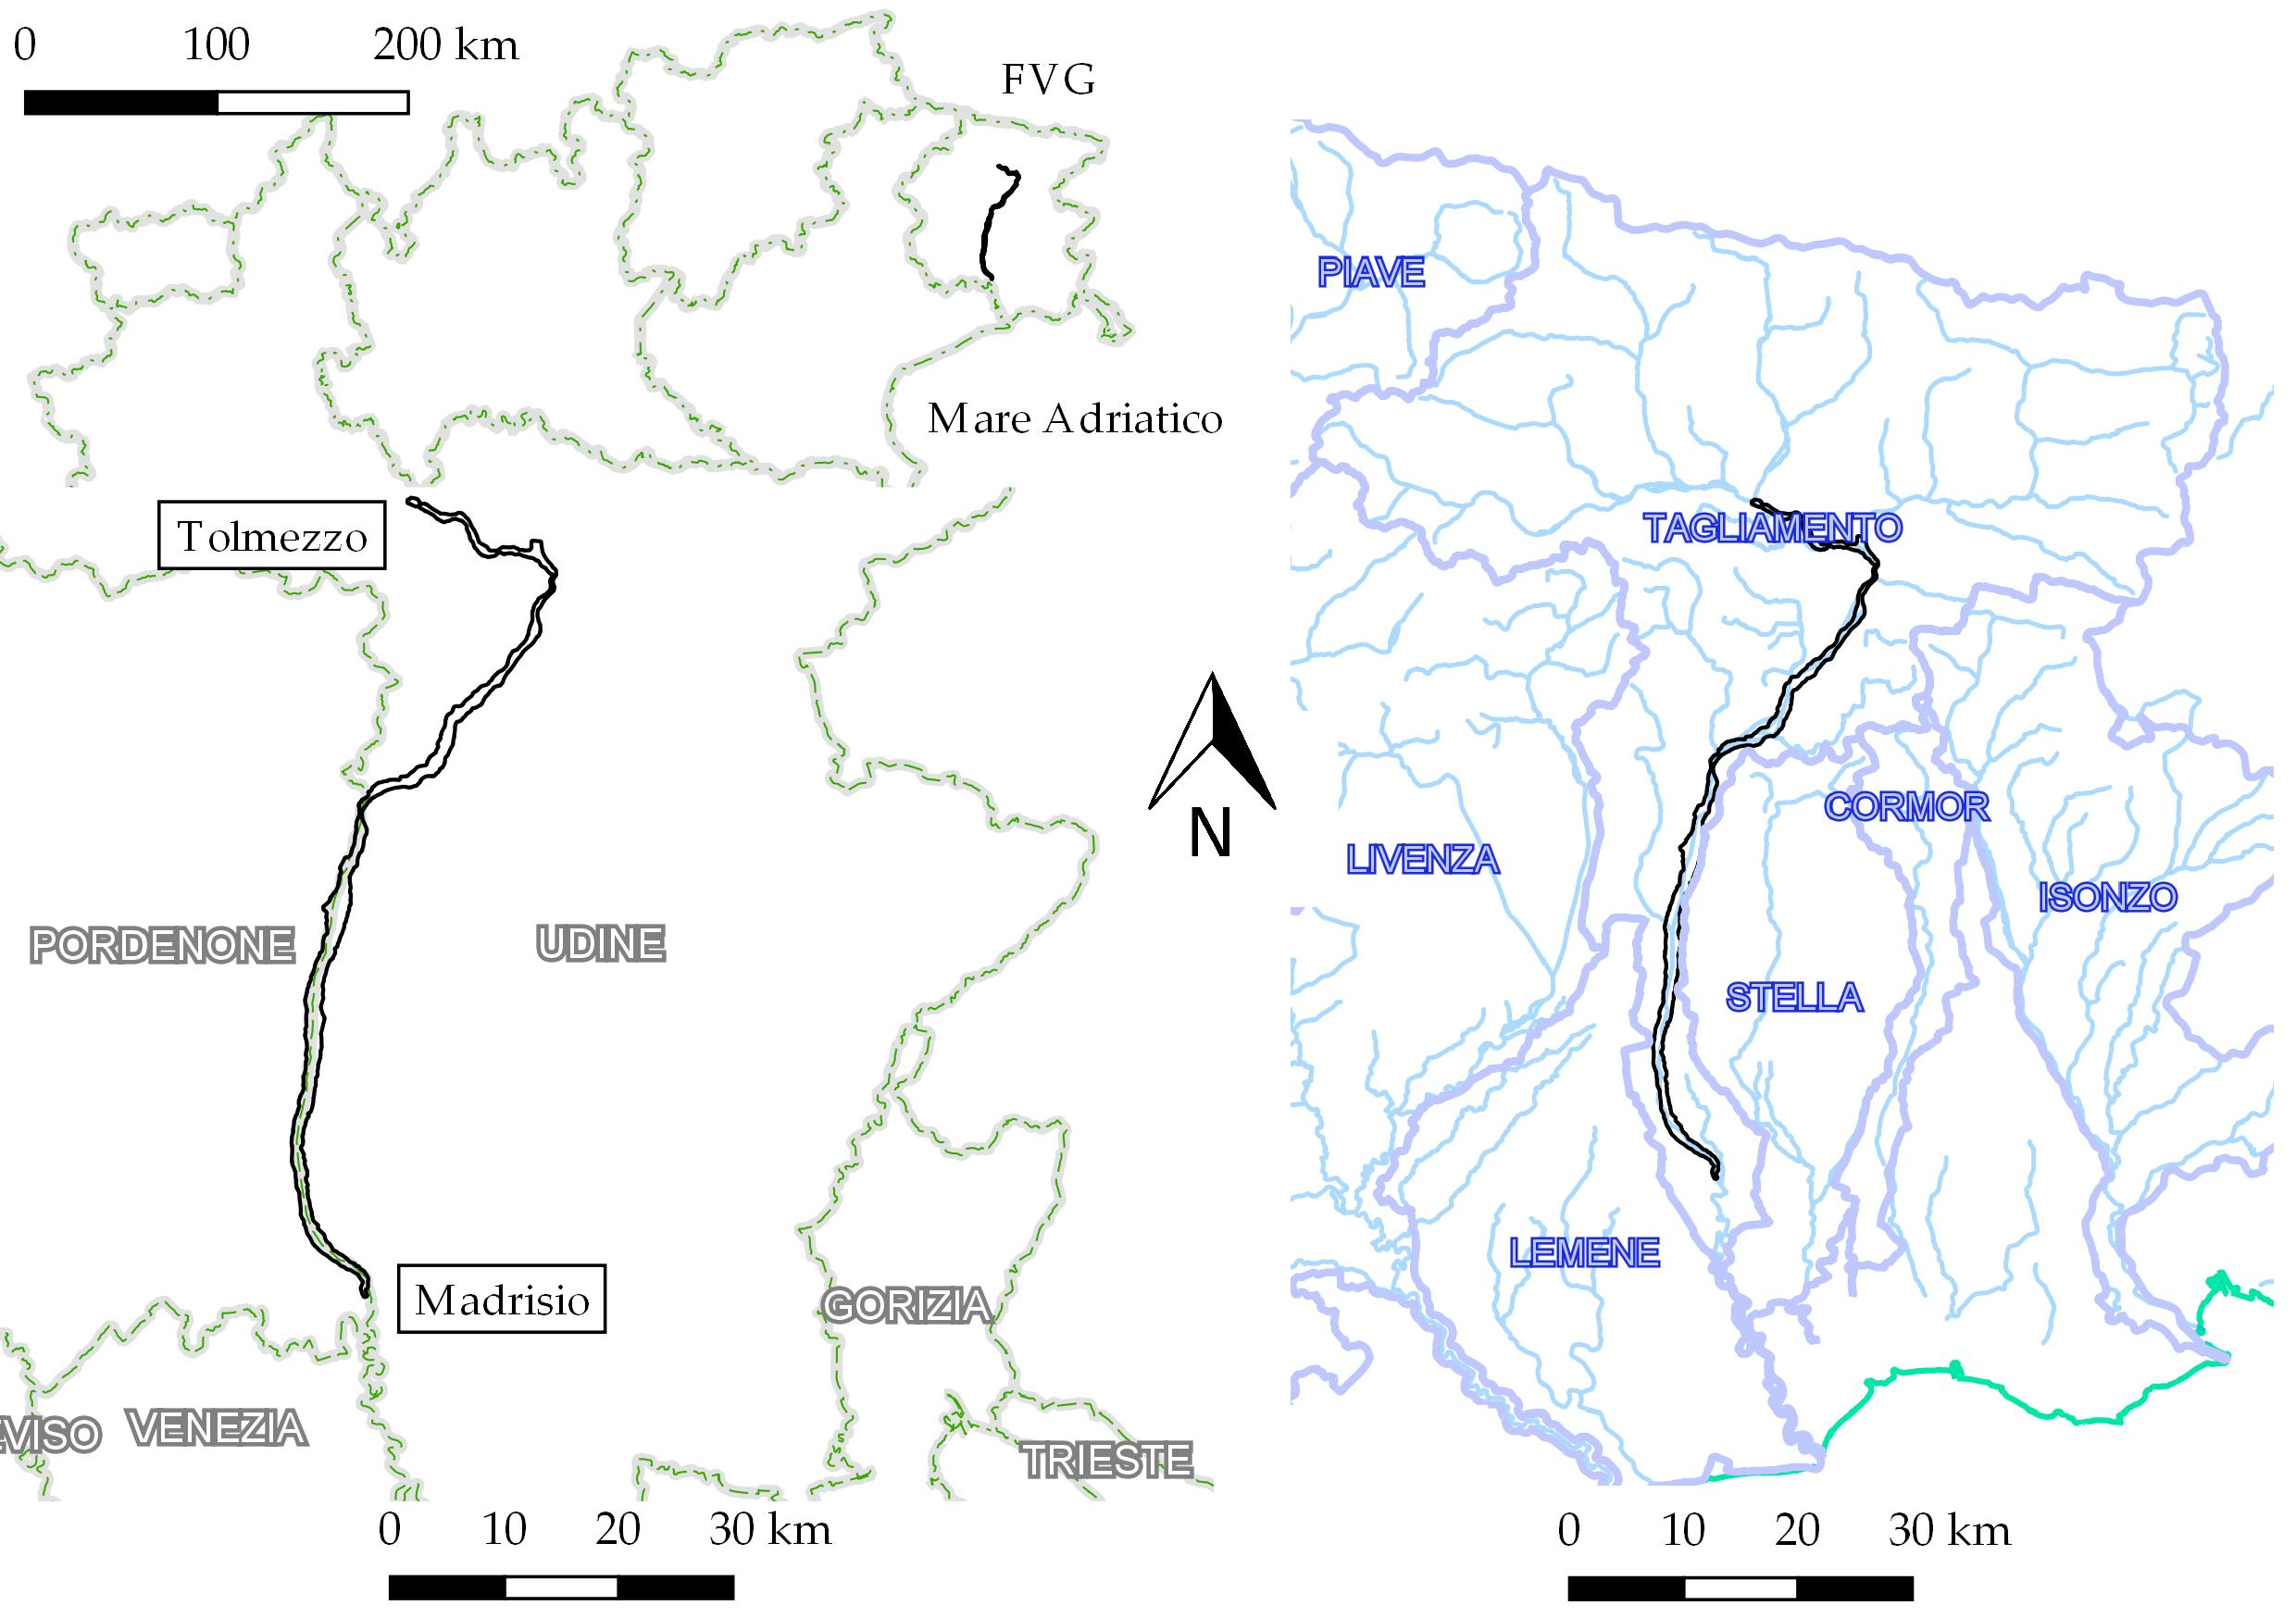
\includegraphics[width=\textwidth]{files/overview.jpeg}
	\caption[inquadramento dell'area di studio]
		{inquadramento dell'area di studio (poligono nero); a sinistra è mostrata l'Italia settentrionale (in alto) e un ingrandimento delle province e degli estremi dell'area di studio (in basso); a destra si vede il bacino idrografico del Tagliamento e di altri fiumi nelle vicinanze (in blu), il reticolo idrografico (in azzurro) e la linea di costa (in verde acqua).}
	\label{fig:overview}
\end{figure}
%
\begin{figure}
	\centering
	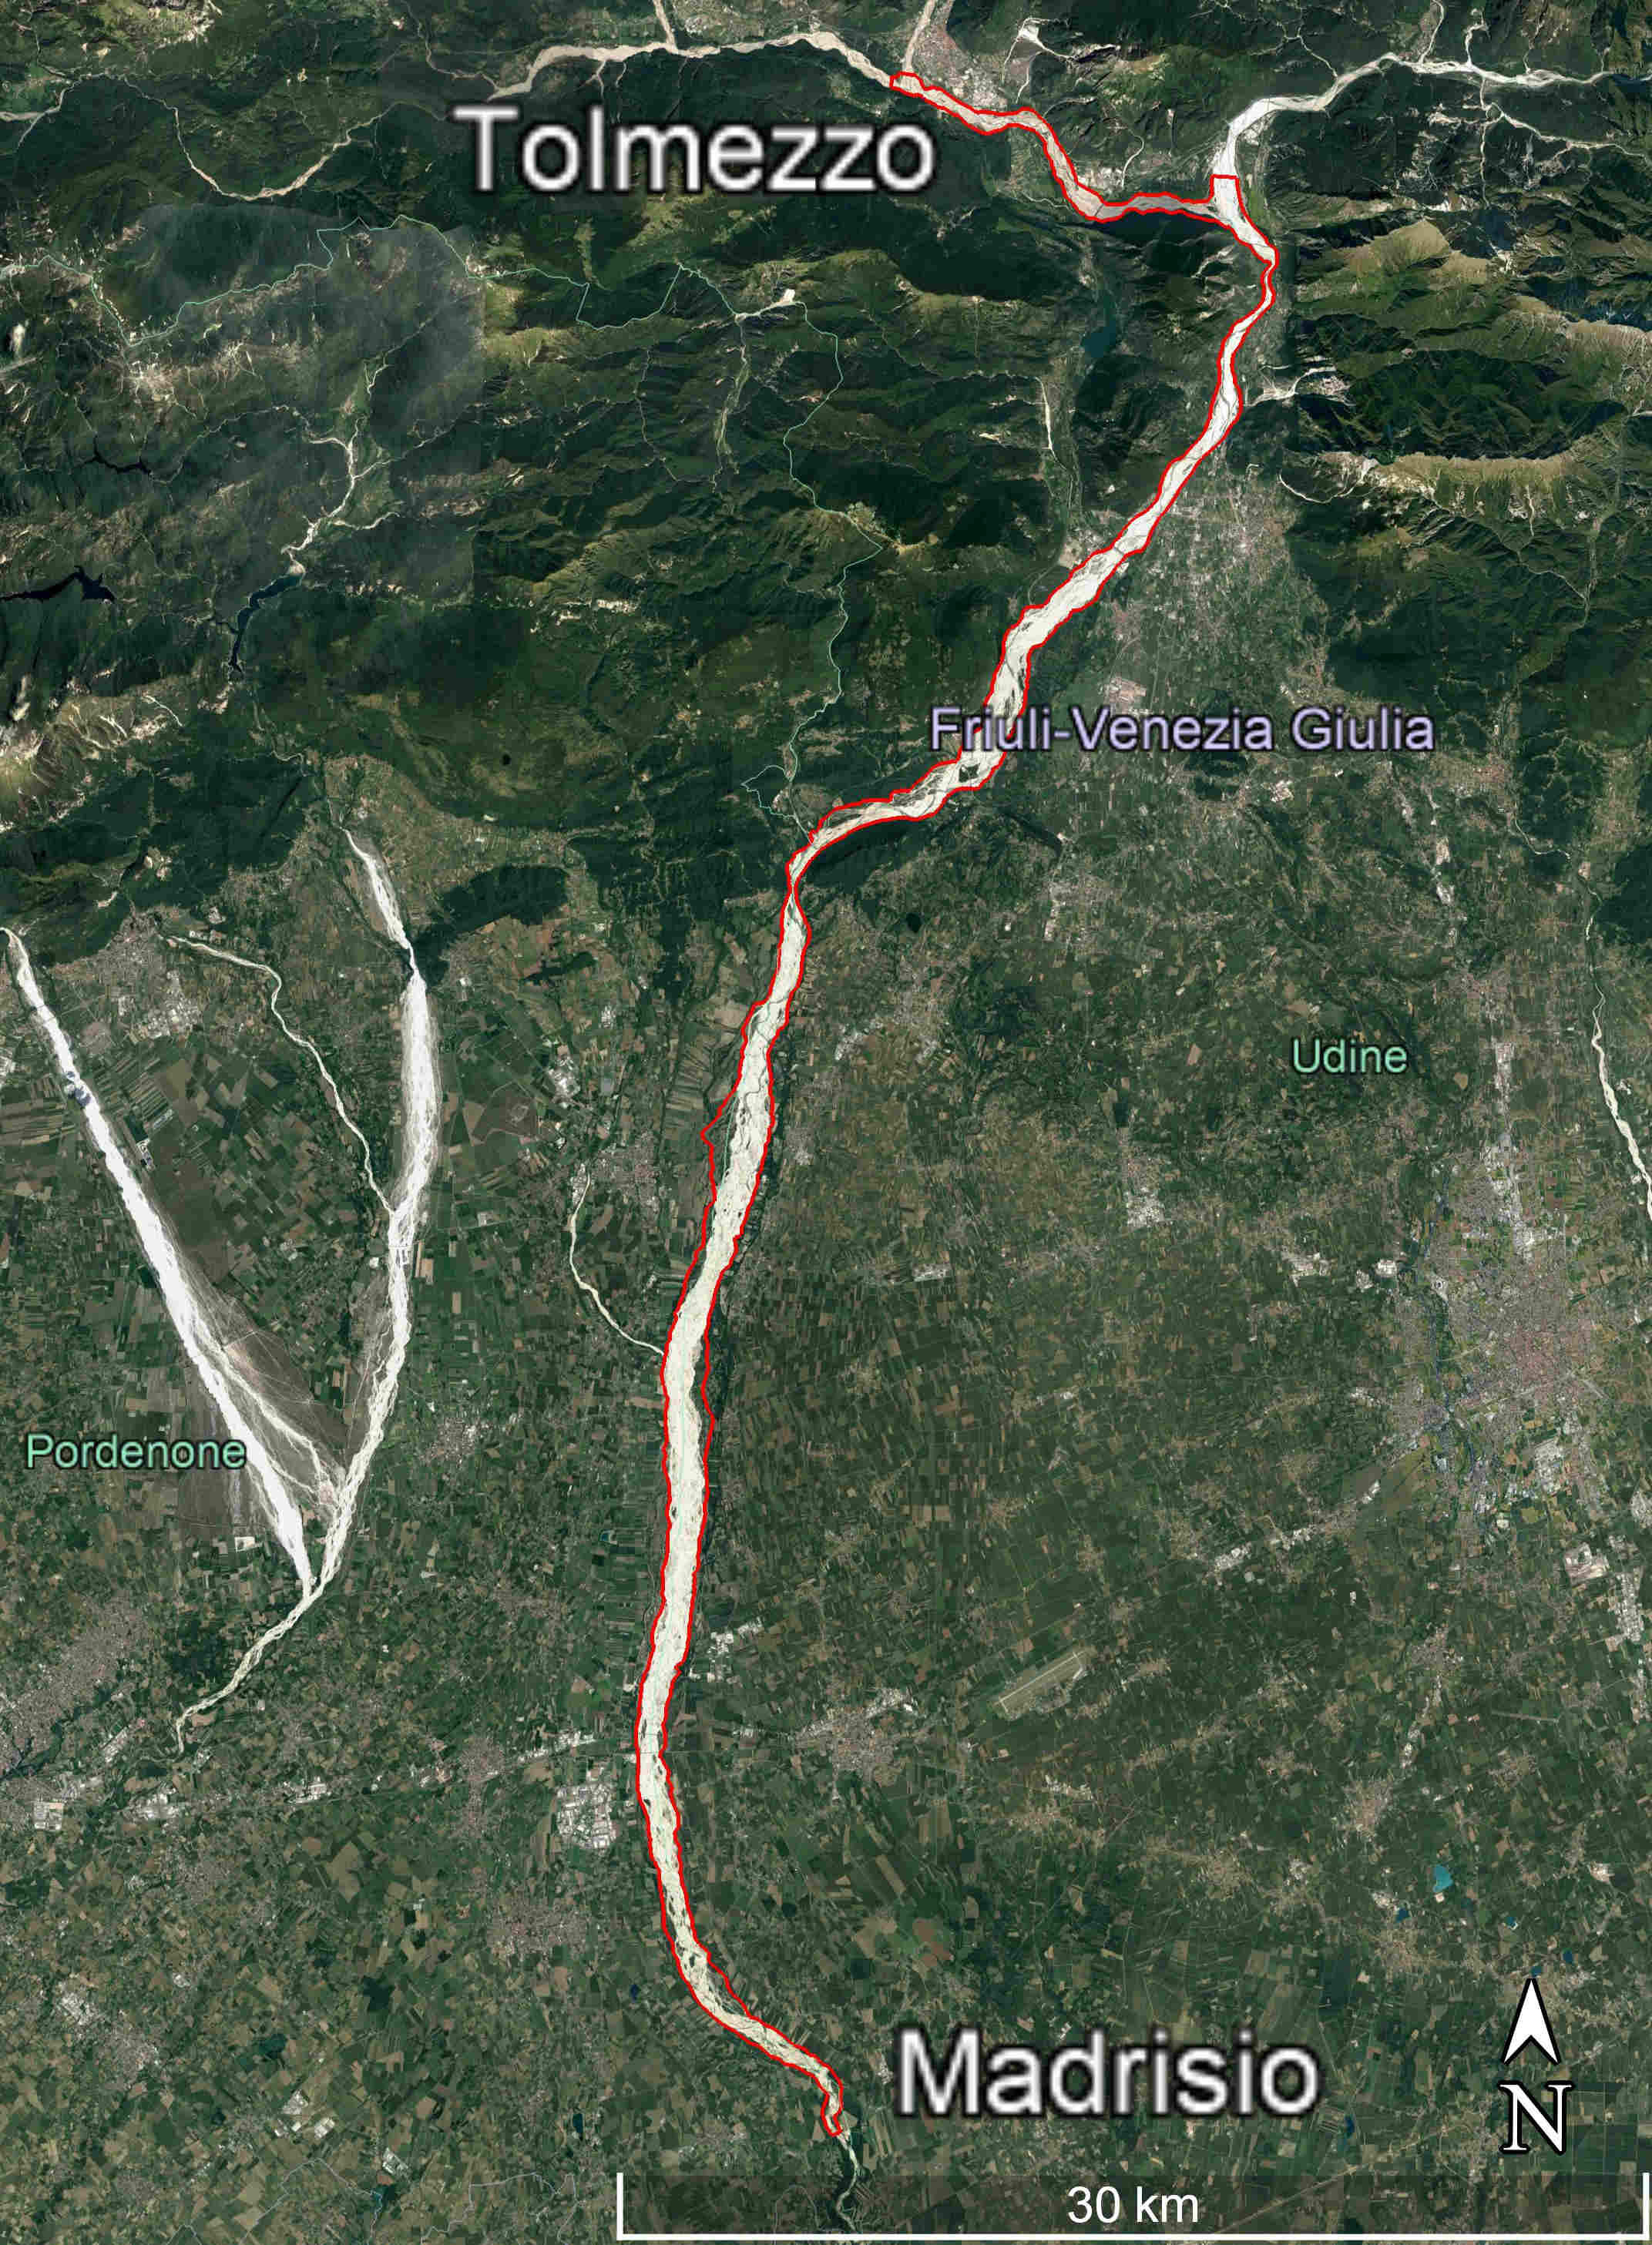
\includegraphics[width=.7\textwidth]{files/overview_gearth.jpg}
	\caption[inquadramento su Google Earth dell'area di studio]{inquadramento su Google Earth dell'area di studio (contornata in rosso).}
	\label{fig:overview-gearth}
\end{figure}



\section{Materiali e metodi}
% materiali
Sono state considerate le bande spettrali del \emph{Near-InfraRed}~(NIR) e del \emph{Red}~(R) nelle immagini satellitari multibande provenienti dalle seguenti missioni:
%
\begin{itemize}
	\item satellite Terra, sensore ASTER Livello~1T (ottenuti in data~21~luglio~2018 \squarecite{data:ASTER});  
		\\
		NIR (Banda~3N)~\SIrange[range-phrase={-}]{0.78}{0.86}{\nano\m}, R (Banda~2)~\SIrange[range-phrase={-}]{0.63}{0.69}{\micro\m};
	\item costellazione Pleiades (\href{https://pleiades.cnes.fr/en/PLEIADES/index.htm}{Centre National d'Etudes Spatiales}\footnote{\texttt{https://pleiades.cnes.fr/en/PLEIADES/index.htm}}); 
		\\
		NIR~\SIrange[range-phrase={-}]{0.74}{0.94}{\micro\m}, R~\SIrange[range-phrase={-}]{0.59}{0.71}{\micro\m};
	\item satellite Sentinel2A, sensore~MSI Livello~1C (ottenuti in data 21~luglio 2018 tramite la API del \href{http://scihub.copernicus.eu/}{Copernicus Open Access Hub}\footnote{\texttt{http://scihub.copernicus.eu/}});
		\\
		NIR (Banda~8)~\SIrange[range-phrase={-}]{0.763}{0.908}{\micro\m}, R (Banda~4)~\SIrange[range-phrase={-}]{0.645}{0.683}{\micro\m}.
\end{itemize}
%

Le ortofoto dell'estate~2011 provengono dal \href{http://www.pcn.minambiente.it/mattm/}{Portale Cartografico Nazionale del Ministero dell'Ambiente e della tutela del territorio e del mare}\footnote{\texttt{http://www.pcn.minambiente.it/mattm/}};
le ortofoto del~2013 sono state effettuate su commissione; 
%
%
le ortofoto del~2017 sono state ottenute da \href{https://www.google.com/earth/}{Google Earth}\footnote{\texttt{https://www.google.com/earth/}}.
\\
I dati idrometrici sono stati forniti dalla \href{http://www.protezionecivile.fvg.it/it/rete-idrometeorologica}{rete idrometeorologica della Protezione Civile della Regione Autonoma Friuli Venezia Giulia}\footnote{\texttt{http://www.protezionecivile.fvg.it/it/rete-idrometeorologica}}.
\\
I grafici \vref{graph:livelli-orto-sat} in \cpageref{graph:livelli-orto-sat} mostrano rispettivamente i livelli idrometrici registrati presso l'idrometro di Villuzza, corrispondente al ponte di Pinzano, e le date di cui si dispongono ortofoto e immagini satellitari (ASTER, Pleiades, Sentinel2, Google~Earth). 
Nel secondo grafico sono riportati solamente i livelli maggiori di~\SI{2}{\m} in quanto, secondo \cite{Bertoldi:2009-2m}, livelli superiori a tale soglia iniziano ad avere effetti di disturbo sulla vegetazione.
La \cpageref{tab:date-orto-sat} mostra le date e la risoluzione delle immagini utilizzate nell'analisi.
%%
\begin{figure}[p]
	\centering
	\begin{tikzpicture}
	%\begin{groupplot}
	\begin{axis}[
		%name = orto-sat,
		axis y line* = right,
		axis x line* = top,
		%height = .3\textwidth,
		width = \textwidth,
		date coordinates in = x,
		%symbolic y coords = {ASTER,PLEIADES,SENTINEL2,G-EARTH},
		xticklabel = {\year-\month-\day},
		xtick = data,
		ytick = data,
		xticklabel style = {
			rotate = 90,
			anchor = near xticklabel
		},
		enlarge x limits = 0.05,
		enlarge y limits = 0.01,
		ylabel = {Fonte},
		ymax = 3.6,
		ymin = -0.1,
		grid = none,
		only marks,
		]
		\addplot table [x=data, y=numero] {graphics/data/data-orto-sat.txt};
	\end{axis}
	%
	\begin{axis}[
		%name = stages,
		%at = {($(orto-sat.south)-(0,2cm)$)},
		%anchor = north,
		axis y line* = left,
		width = \textwidth,
		date coordinates in = x,
		xticklabel = {\year-\month-\day},
		xticklabel style = {
			rotate = 45,
			anchor = near xticklabel
		},
		enlarge x limits = 0.05,
		enlarge y limits = 0.01,
		ymax = 3.6,
		ymin = -0.1,
		ylabel = {Livello idrometrico},
		grid = major,
		no markers,
		]
		\addplot table [x=data, y=media-gg] {graphics/data/Dati_Villuzza.csv};
	\end{axis}
\end{tikzpicture}
	\tikzsetnextfilename{livelli_2m+imm}
\begin{tikzpicture}
	\begin{axis}[
		width = \textwidth,
		height = 0.5\textwidth,
		date coordinates in = x,
		date ZERO = 2000-01-01,
		xticklabel = {$\year$},
		xticklabel style = {
			rotate = 80,
			anchor = near xticklabel
		},
		xtick distance = 732,
		enlarge x limits = 0.05,
		enlarge y limits = 0.01,
		ymax = 3.7,
		ymin = 1.95,
		ylabel = {Livello idrometrico \si{[\m]}},
		grid = major,
		]
		\addplot+ 
			[red, mark=x, semithick, style=solid, mark=x]
			coordinates {(2000-09-17, 2)(2000-09-17, 3.7)};
		\addplot+ 
			[red, semithick, style=solid, mark=x]
			coordinates {(2001-06-07, 2)(2001-06-07, 3.7)};
		\addplot+
        	[red, semithick, style=solid, mark=x]
        	coordinates {(2002-05-18, 2)(2002-05-18, 3.7)};
		\addplot+
        	[red, semithick, style=solid, mark=x]
        	coordinates {(2002-06-12, 2)(2002-06-12, 3.7)};
		\addplot+
        	[red, semithick, style=solid, mark=x]
        	coordinates {(2003-06-22, 2)(2003-06-22, 3.7)};
		\addplot+
        	[red, semithick, style=solid, mark=x]
        	coordinates {(2004-10-14, 2)(2004-10-14, 3.7)};
		\addplot+
        	[green, semithick, style=solid, mark=x]
        	coordinates {(2005-05-01, 2)(2005-05-01, 3.7)};
		\addplot+
        	[red, semithick, style=solid, mark=x]
        	coordinates {(2005-08-30, 2)(2005-08-30, 3.7)};
		\addplot+
        	[red, semithick, style=solid, mark=x]
        	coordinates {(2006-07-16, 2)(2006-07-16, 3.7)};
		\addplot+
        	[red, semithick, style=solid, mark=x]
        	coordinates {(2007-09-21, 2)(2007-09-21, 3.7)};
		\addplot+
        	[red, semithick, style=solid, mark=x]
        	coordinates {(2008-07-05, 2)(2008-07-05, 3.7)};
		\addplot+
        	[red, semithick, style=solid, mark=x]
        	coordinates {(2009-07-08, 2)(2009-07-08, 3.7)};
		\addplot+
        	[green, semithick, style=solid, mark=x]
        	coordinates {(2010-08-01, 2)(2010-08-01, 3.7)};
		\addplot+
        	[red, semithick, style=solid, mark=x]
        	coordinates {(2010-09-29, 2)(2010-09-29, 3.7)};
		\addplot+
        	[green, semithick, style=solid, mark=x]
        	coordinates {(2011-07-01, 2)(2011-07-01, 3.7)};
		\addplot+
        	[red, semithick, style=solid, mark=x]
        	coordinates {(2012-08-01, 2)(2012-08-01, 3.7)};
		\addplot+
        	[red, semithick, style=solid, mark=x]
        	coordinates {(2013-09-05, 2)(2013-09-05, 3.7)};
		\addplot+
        	[green, semithick, style=solid, mark=x]
        	coordinates {(2013-10-22, 2)(2013-10-22, 3.7)};
		\addplot+
        	[red, semithick, style=solid, mark=x]
        	coordinates {(2014-09-08, 2)(2014-09-08, 3.7)};
		\addplot+
        	[black, semithick, style=solid, mark=x]
        	coordinates {(2014-10-31, 2)(2014-10-31, 3.7)};
       	\addplot+
        	[black, semithick, style=solid, mark=x]
        	coordinates {(2015-08-13, 2)(2015-08-13, 3.7)};
		\addplot+
        	[cyan, semithick, style=solid, mark=x]
        	coordinates {(2015-09-12, 2)(2015-09-12, 3.7)};
		\addplot+
        	[cyan, semithick, style=solid, mark=x]
        	coordinates {(2015-10-22, 2)(2015-10-22, 3.7)};
		\addplot+
        	[cyan, semithick, style=solid, mark=x]
        	coordinates {(2016-09-13, 2)(2016-09-13, 3.7)};
		\addplot+
        	[cyan, semithick, style=solid, mark=x]
        	coordinates {(2017-04-21, 2)(2017-04-21, 3.7)};
		\addplot+
        	[cyan, semithick, style=solid, mark=x]
        	coordinates {(2017-06-13, 2)(2017-06-13, 3.7)};
		\addplot+
        	[green, semithick, style=solid, mark=x]
        	coordinates {(2017-07-07, 2)(2017-07-07, 3.7)};
       	\addplot+
        	[violet, semithick, style=solid, mark=x]
        	coordinates {(2018-06-15, 2)(2018-06-15, 3.7)};
		\addplot+
        	[cyan, semithick, style=solid, mark=x]
        	coordinates {(2018-09-16, 2)(2018-09-16, 3.7)};
		\addplot+
        	[blue, solid, no markers]
        	table [x=data, y=media-gg] {graphics/data/Dati_Villuzza.csv};
	\end{axis}
\end{tikzpicture}
	\caption[livelli idrometrici e foto aeree - satellitari]{in alto il livello idrometrico (in blu) presso l'idrometro di Villuzza. 
	In basso un ingrandimento per i livelli superiori a~\SI{2}{\m}. Le linee indicano le immagini satellitari e le ortofoto considerate (ASTER in magenta, ortofoto in arancione, Pleiades in verde~acqua, Sentinel2 in azzurro, G-Earth in verde).}
	\label{graph:livelli-orto-sat}
\end{figure}
%%%
\begin{table}[p]
	\centering
	\begin{tabular}{c c S[table-format=2.2]}
		\toprule
		Data		&	Fonte		&	\multicolumn{1}{c}{Ris \si{[\m]}}	\\
		\midrule	
		2000-09-17		&	ASTER		&	15	\\
		2001-06-07		&	ASTER		&	15	\\
		2001-12-09		&	ASTER		&	15	\\
		2002-05-18		&	ASTER		&	15	\\
		2002-06-12		&	ASTER		&	15	\\
		2003-06-22		&	ASTER		&	15	\\
		2003-11-29		&	ASTER		&	15	\\
		2004-10-14		&	ASTER		&	15	\\
		2005-08-30		&	ASTER		&	15	\\
		2006-07-16		&	ASTER		&	15	\\
		2007-09-21		&	ASTER		&	15	\\
		2008-07-05		&	ASTER		&	15	\\
		2009-07-08		&	ASTER		&	15	\\
		2010-09-29		&	ASTER		&	15	\\
		2011-06-26/07-02	&	Ortofoto	&	1	\\
		2012-08-01		&	ASTER		&	15	\\
		2013-09-05		&	ASTER		&	15	\\
		2013-10-22		&	Ortofoto	&	0.2	\\
		2014-09-08		&	ASTER		&	15	\\
		2014-10-31		&	Pleiades	&	0.5	\\
		2015-09-11		&	ASTER		&	15	\\
		2015-09-29		&	Sentinel2	&	10	\\
		2016-09-13		&	Sentinel2	&	10	\\
		2017-04-21		&	Sentinel2	&	10	\\
		2017-06-26/08-02	&	G-Earth	&	0.45	\\
		\bottomrule
	\end{tabular}
	\caption{data e risoluzione delle immagini satellitari e delle ortofoto utilizzate.}
	\label{tab:date-orto-sat}
\end{table}



% strumenti
\medskip
Per eseguire le analisi sulle immagini aeree e satellitari sono stati utilizzati i GIS GRASS \squarecite{soft:GRASS} e QGIS \squarecite{soft:QGIS}. 
Per il download e il pre-processing delle immagini satellitari è stato usato SCP, plugin di QGIS \squarecite{soft:SCP}. 
Per il download delle ortofoto del~2017 si è utilizzato \href{https://github.com/sourcepole/qgis-openlayers-plugin}{OpenLayers}\footnote{\texttt{https://github.com/sourcepole/qgis-openlayers-plugin}}, plugin di QGIS.

%----------------------------------------------------------



\chapter{Vegetazione e piene}
F\section{Quantità di vegetazione in alveo}
Si è misurata l'area della vegetazione presente in alveo e nella parte di floodplain soggetta a forti disturbi (erosione e distacco di isole); 
a tal fine si è seguito l'approccio di altri autori in analisi simili eseguite su immagini ASTER e LandSat~TM \squarecites{Bertoldi:2011-ASTER}{Henshaw:2013-LandSat}.
%
\begin{description}
	\item[Maschera computazionale] 
	Dapprima è stata individuata manualmente una maschera di calcolo che comprendesse l'alveo attivo e la parte di piana alluvionale che è stata erosa quando coinvolta nelle piene; 
	tale maschera si estende da Tolmezzo al ponte di Madrisio
	(\vref{fig:esempio-maschera}). 
	Applicandola, il dominio computazionale è stato ridotto a comprendere l'inviluppo degli alvei attivi che si sono succeduti dall'immagine del~2000 all'ortofoto del~2017.
	%
	\begin{figure}[t]
		\centering
		\begin{subfigure}[b]{0.296\textwidth}
			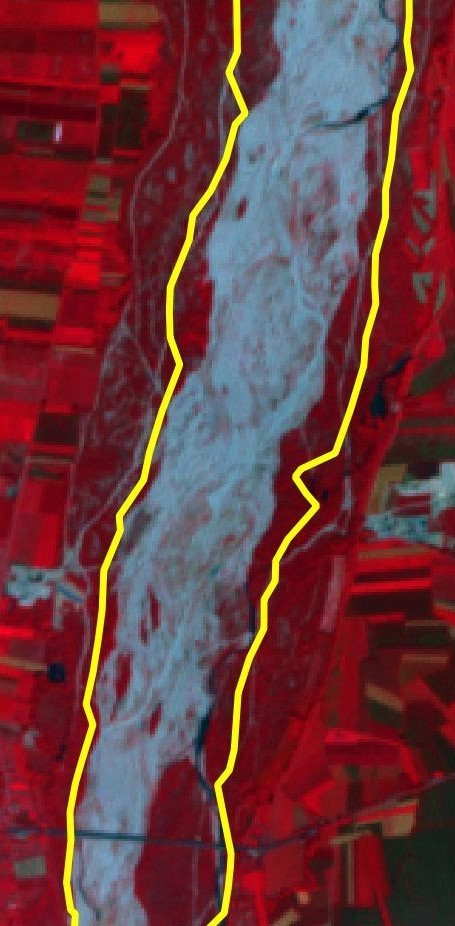
\includegraphics[width=\textwidth]{files/esempio_mask_2000_09_17.jpeg}
			\caption{ASTER 2000-09-17.}
		\end{subfigure}
		\qquad
		\begin{subfigure}[b]{0.30\textwidth}
			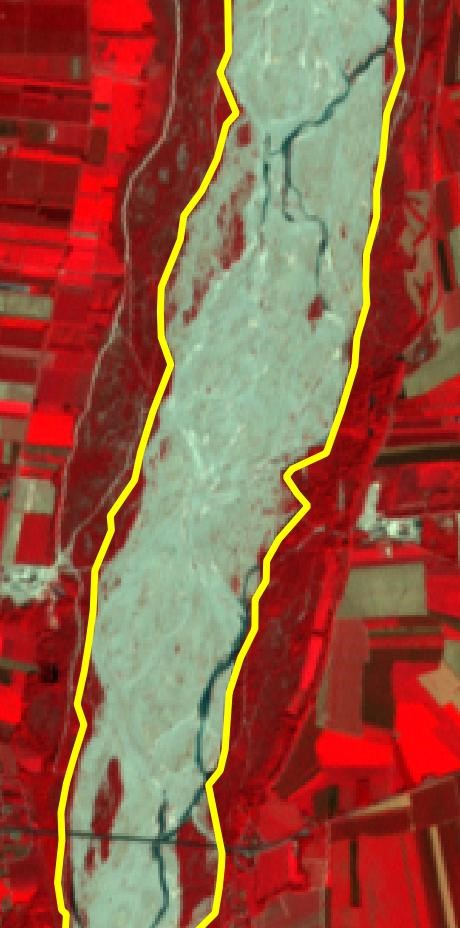
\includegraphics[width=\textwidth]{files/esempio_mask_2015_09_11.jpeg}
			\caption{ASTER 2015-09-11.}
		\end{subfigure}
		\caption[definizione della maschera per limitare il dominio computazionale]
			{esempio in cui si vede come la maschera utilizzata per limitare il dominio computazionale (in giallo) sia il risultato dell'inviluppo degli alvei attivi che si sono modificati nel tempo; le immagini sono in falsi colori (IR-R-G).}
		\label{fig:esempio-maschera}
	\end{figure}
	%
	%
	\item[NDVI] 
	In questa area è stato calcolato il \emph{Normalized Difference Vegetation Index} (NDVI) grazie alle bande del \emph{Near Infrared} (NIR) e del \emph{Red} (R)
	%
	\begin{equation}
		%\notag
		NDVI = \frac{NIR - R}{NIR + R} \quad .
		\label{eq:ndvi}
	\end{equation}
	%
	%
	\item[Aree campione]
	\`{E} stata effettuata una digitalizzazione manuale di alcune aree campione per le immagini ASTER del~2005-08-30 ($\sim 70$) e del~2012-08-01 ($\sim 100$), l'immagine Plaiades del~2014-10-31 ($\sim 40$) e l'immagine Sentinel2 del~2017-04-21 ($\sim 45$) (\vref{fig:esempio-aree-campione}).
	Sono state selezionate immagini per ogni satellite poiché ciascuno è sensibile a bande leggermente diverse; si sono osservate due immagini ASTER dato il grande numero di immagini disponibili da questo sensore scegliendo quelle con minor nuvolosità.
	\\
	Queste aree campione sono state suddivise in tre classi: vegetazione, alveo attivo e canale.
	%
	\begin{figure}[ht]
		\centering
		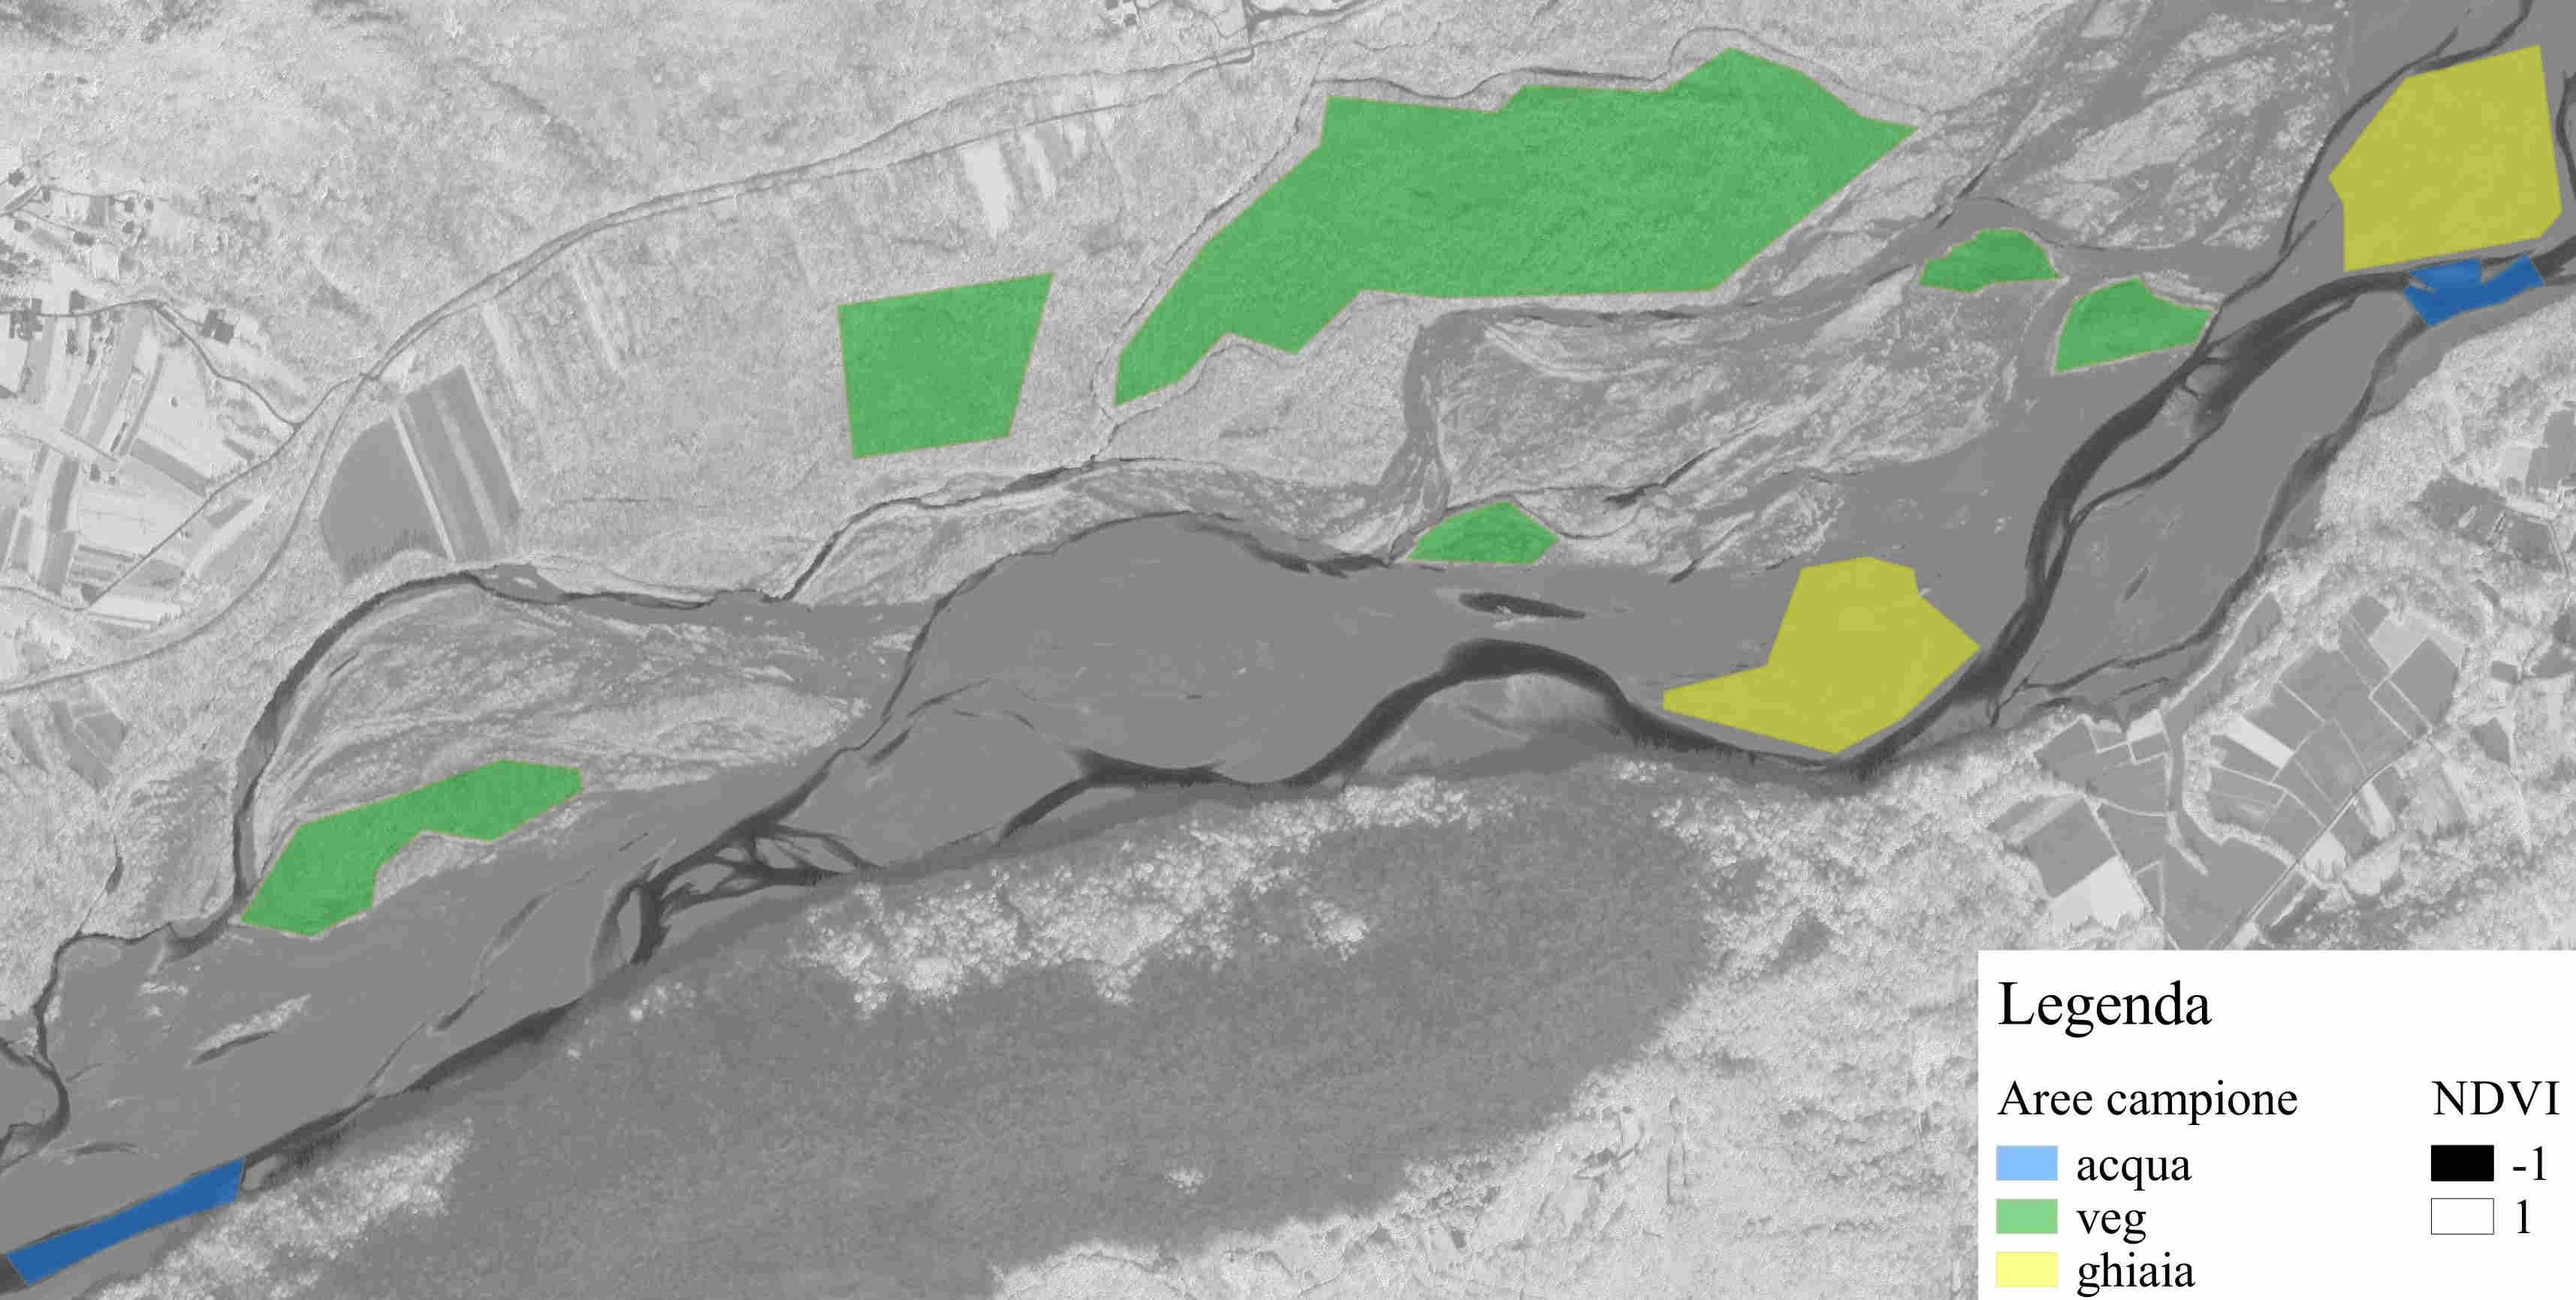
\includegraphics[width=\textwidth]{files/esempio_aree_campione_2014_10_31.jpeg}
		\caption[esempio di aree campione per calcolare la distribuzione dell'NDVI]{esempio di digitalizzazione di alcune aree campione per l'immagine Pleiades del~2014-10-31; sullo sfondo la mappa dell'NDVI.}
		\label{fig:esempio-aree-campione}
	\end{figure}
	%
	%
	\item[Percentili aree campione]
	Per ogni immagine si è osservata la distribuzione dell'NDVI in ogni classe (\vref{graph:percentili}).
	% 
	\begin{figure}[ht]
		\centering
		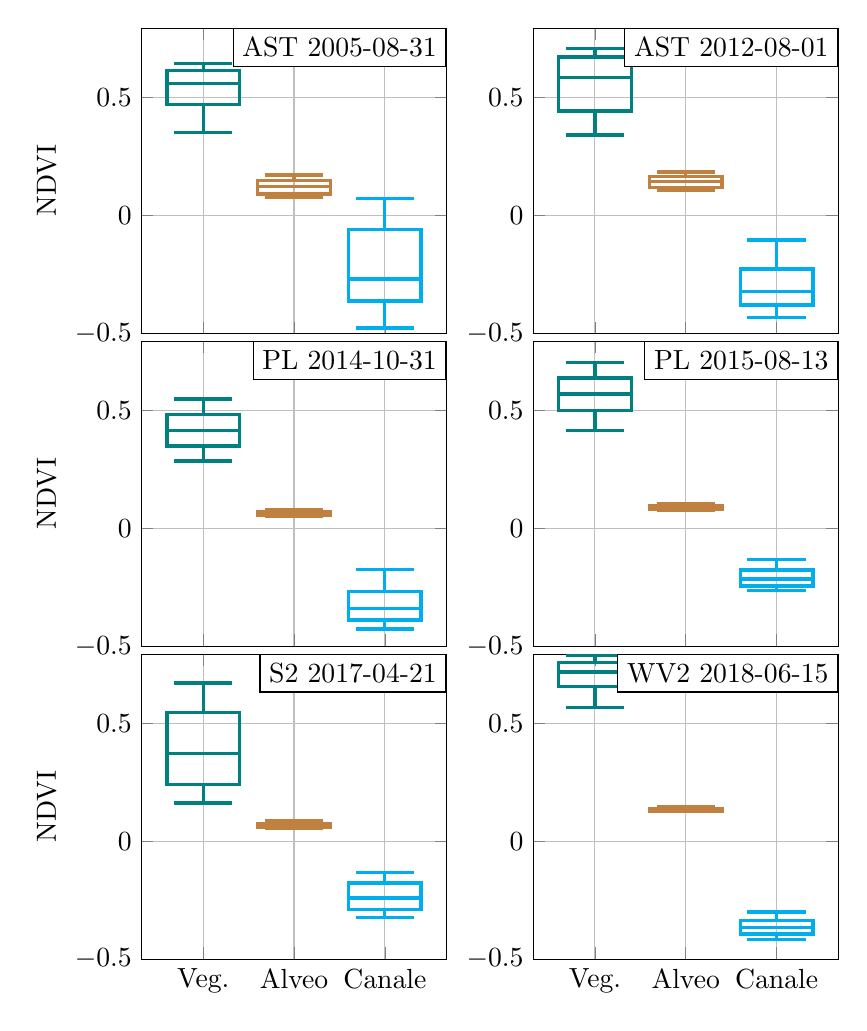
\begin{tikzpicture}
	\begin{groupplot}[
		group style = {
			group size = 2 by 3,
			ylabels at = edge left,
			x descriptions at = edge bottom,
			horizontal sep = 1.1cm,
			vertical sep = 0.1cm,
		},
		width = 0.45\textwidth,
		height = 0.45\textwidth,
		ylabel = NDVI,
		boxplot/draw direction = y,
		xtick = {1,2,3},
		xticklabels = {Veg., Alveo, Canale},
		ymax = 0.795,
		ymin = -0.50,
		grid = major,
	]
	\nextgroupplot % ASTER 2005-08-31
		\addplot+ [ % vegetazione
			teal, very thick,
			boxplot prepared = {
				lower whisker = 0.353656,
				lower quartile = 0.470411,
				median = 0.560063,
				upper quartile = 0.614701,
				upper whisker = 0.644957,
				},
        	]
        	coordinates {};
		\addplot+ [ % alveo attivo
			brown, very thick,
			boxplot prepared = {
				lower whisker = 0.077472,
				lower quartile = 0.091653,
				median = 0.122488,
				upper quartile = 0.149573,
				upper whisker = 0.171459,
				},
        	]
        	coordinates {};
		\addplot+ [ % canale
			cyan, very thick,
			boxplot prepared = {
				lower whisker = -0.477885,
				lower quartile = -0.362798,
				median = -0.269905,
				upper quartile = -0.058787,
				upper whisker = 0.072414,
				},
        	]
        	coordinates {};
        \node [fill = white, draw = black, anchor = north east] 
        	at (axis description cs: 1,1) {AST 2005-08-31};
	%------------------------------------------------------
	\nextgroupplot % ASTER 2012-08-01
		\addplot+ [ % vegetazione
			teal, very thick,
			boxplot prepared = {
				lower whisker = 0.341613,
				lower quartile = 0.444200,
				median = 0.586294,
				upper quartile = 0.672889,
				upper whisker = 0.709027,
				},
        	]
        	coordinates {};
		\addplot+ [ % alveo attivo
			brown, very thick,
			boxplot prepared = {
				lower whisker = 0.10506,
				lower quartile = 0.117969,
				median = 0.143631,
				upper quartile = 0.16549,
				upper whisker = 0.184871,
				},
        	]
        	coordinates {};
		\addplot+ [ % canale
			cyan, very thick,
			boxplot prepared = {
				lower whisker = -0.432201,
				lower quartile = -0.379825,
				median = -0.322239,
				upper quartile = -0.226459,
				upper whisker = -0.103914,
				},
        	]
        	coordinates {};
        \node [fill = white, draw = black, anchor = north east] 
        	at (axis description cs: 1,1) {AST 2012-08-01};
	%------------------------------------------------------
	\nextgroupplot % Pleiades 2014-10-31
		\addplot+ [ % vegetazione
			teal, very thick,
			boxplot prepared = {
				lower whisker = 0.286467,
				lower quartile = 0.350238,
				median = 0.415502,
				upper quartile = 0.483495,
				upper whisker = 0.549505,
				},
        	]
        	coordinates {};
		\addplot+ [ % alveo attivo
			brown, very thick,
			boxplot prepared = {
				lower whisker = 0.049796,
				lower quartile = 0.055794,
				median = 0.063049,
				upper quartile = 0.07173,
				upper whisker = 0.081427,
				},
        	]
        	coordinates {};
		\addplot+ [ % canale
			cyan, very thick,
			boxplot prepared = {
				lower whisker = -0.426415,
				lower quartile = -0.387978,
				median = -0.338308,
				upper quartile = -0.266515,
				upper whisker = -0.175373,
				},
        	]
        	coordinates {};
        \node [fill = white, draw = black, anchor = north east] 
        	at (axis description cs: 1,1) {PL 2014-10-31};
	%------------------------------------------------------
	\nextgroupplot % Pleiades 2015-08-13
		\addplot+ [ % vegetazione
			teal, very thick,
			boxplot prepared = {
				lower whisker = 0.415693,
				lower quartile = 0.5,
				median = 0.570359,
				upper quartile = 0.638507,
				upper whisker = 0.704044		
,
				},
        	]
        	coordinates {};
		\addplot+ [ % alveo attivo
			brown, very thick,
			boxplot prepared = {
				lower whisker = 0.075052,
				lower quartile = 0.080858,
				median = 0.087921,
				upper quartile = 0.096031,
				upper whisker = 0.106198,
				},
        	]
        	coordinates {};
		\addplot+ [ % canale
			cyan, very thick,
			boxplot prepared = {
				lower whisker = -0.262599,
				lower quartile = -0.244228,
				median = -0.214393,
				upper quartile = -0.176471,
				upper whisker = -0.132762,
				},
        	]
        	coordinates {};
        \node [fill = white, draw = black, anchor = north east] 
        	at (axis description cs: 1,1) {PL 2015-08-13};
	%------------------------------------------------------
	\nextgroupplot % Sentinel2 2017-04-21
		\addplot+ [ % vegetazione
			teal, very thick,
			boxplot prepared = {
				lower whisker = 0.163722,
				lower quartile = 0.241916,
				median = 0.374344,
				upper quartile = 0.548241,
				upper whisker = 0.672782,
				},
        	]
        	coordinates {};
		\addplot+ [ % alveo attivo
			brown, very thick,
			boxplot prepared = {
				lower whisker = 0.056176,
				lower quartile = 0.061278,
				median = 0.067681,
				upper quartile = 0.076396,
				upper whisker = 0.089304,
				},
        	]
        	coordinates {};
		\addplot+ [ % canale
			cyan, very thick,
			boxplot prepared = {
				lower whisker = -0.322237,
				lower quartile = -0.288822,
				median = -0.239533,
				upper quartile = -0.177094,
				upper whisker = -0.131119,
				},
        	]
        	coordinates {};
        \node [fill = white, draw = black, anchor = north east] 
        	at (axis description cs: 1,1) {S2 2017-04-21};
	%------------------------------------------------------
	\nextgroupplot % WorldView2 2018-06-15
		\addplot+ [ % vegetazione
			teal, very thick,
			boxplot prepared = {
				lower whisker = 0.569665,
				lower quartile = 0.657917,
				median = 0.719523,
				upper quartile = 0.759148,
				upper whisker = 0.791594,
				},
        	]
        	coordinates {};
		\addplot+ [ % alveo attivo
			brown, very thick,
			boxplot prepared = {
				lower whisker = 0.126214,
				lower quartile = 0.129661,
				median = 0.13373,
				upper quartile = 0.138542,
				upper whisker = 0.149326,
				},
        	]
        	coordinates {};
		\addplot+ [ % canale
			cyan, very thick,
			boxplot prepared = {
				lower whisker = -0.416974,
				lower quartile = -0.392405,
				median = -0.365385,
				upper quartile = -0.335135,
				upper whisker = -0.29979,
				},
        	]
        	coordinates {};
        \node [fill = white, draw = black, anchor = north east] 
        	at (axis description cs: 1,1) {WV2 2018-06-15};
	\end{groupplot}
\end{tikzpicture}

		\caption[boxplot dell'NDVI nelle aree campione in quattro immagini satellitari]{boxplot dell'NDVI nelle aree campione in quattro immagini satellitari; i baffi indicano il 10mo e il 90mo percentile, gli estremi della scatola rappresentano il 25mo e il 75mo percentile, la linea nella scatola è la mediana.}
		\label{graph:percentili}
	\end{figure}
	%
	%
	\item[Soglie NDVI] 
	Da tali grafici sono state ottenute delle soglie di NDVI per classificare le immagini satellitari (\vref{tab:ndvi-soglia}); per l'immagine WorldView2 la soglia che distingue vegetazione da alveo attivo è maggiore. Le soglie sono in accordo con quanto riportato in letteratura \squarecite{Bertoldi:2011-ASTER}.
	%
	\begin{table}[ht]
		\centering
		\begin{tabular}{
			c 
			S[table-format=1.1]@{\,}
			c@{\,}
			c@{\,}
			c@{\,}
			S[table-format=1.1]
			S[table-format=1.1]@{\,}
			c@{\,}
			c@{\,}
			c@{\,}
			S[table-format=1.1]
			}
			\toprule
			&	\multicolumn{5}{c}{\textbf{Soglie AST PL S2}}	&	\multicolumn{5}{c}{\textbf{Soglie WV2}}	\\
			\midrule
			Vegetazione		&	0.2	&	$\leq$	&	NDVI	&			&		& 	0.3	&	$\leq$	&	NDVI	&			& 	\\
			Alveo attivo	&	0.0	&	$\leq$	&	NDVI	&	$<$		&	0.2	&	0.0	&	$\leq$	&	NDVI	&	$<$		&	0.3\\
			Canale			&		&			&	NDVI	&	$<$		&	0.0	&		&			&	NDVI	&	$<$		&	0.0\\
			\bottomrule
		\end{tabular}
		\caption[soglie NDVI]{soglie di NDVI per la classificazione delle immagini satellitari.}
		\label{tab:ndvi-soglia}
	\end{table}
	%
	%
	\item[Divisione in 23 tratti]
	La maschera di calcolo è stata suddivisa manualmente in 23~tratti con 22~sezioni al fine di avere un maggior dettaglio spaziale delle dinamiche di vegetazione (\vref{fig:23-tratti}). 
	Questi tratti sono stati selezionati in modo da possedere caratteristiche omogenee per portata e crescita della vegetazione; 
	pertanto confluenze di immissari, bruschi restringimenti o allargamenti, inizio di pronunciato \emph{upwelling} o \emph{downwelling} ed evidenti cambiamenti di morfologia fluviale sono stati gli elementi per individuare le 22~sezioni che determinano i 23~tratti.
	%
	\begin{figure}
		\centering
		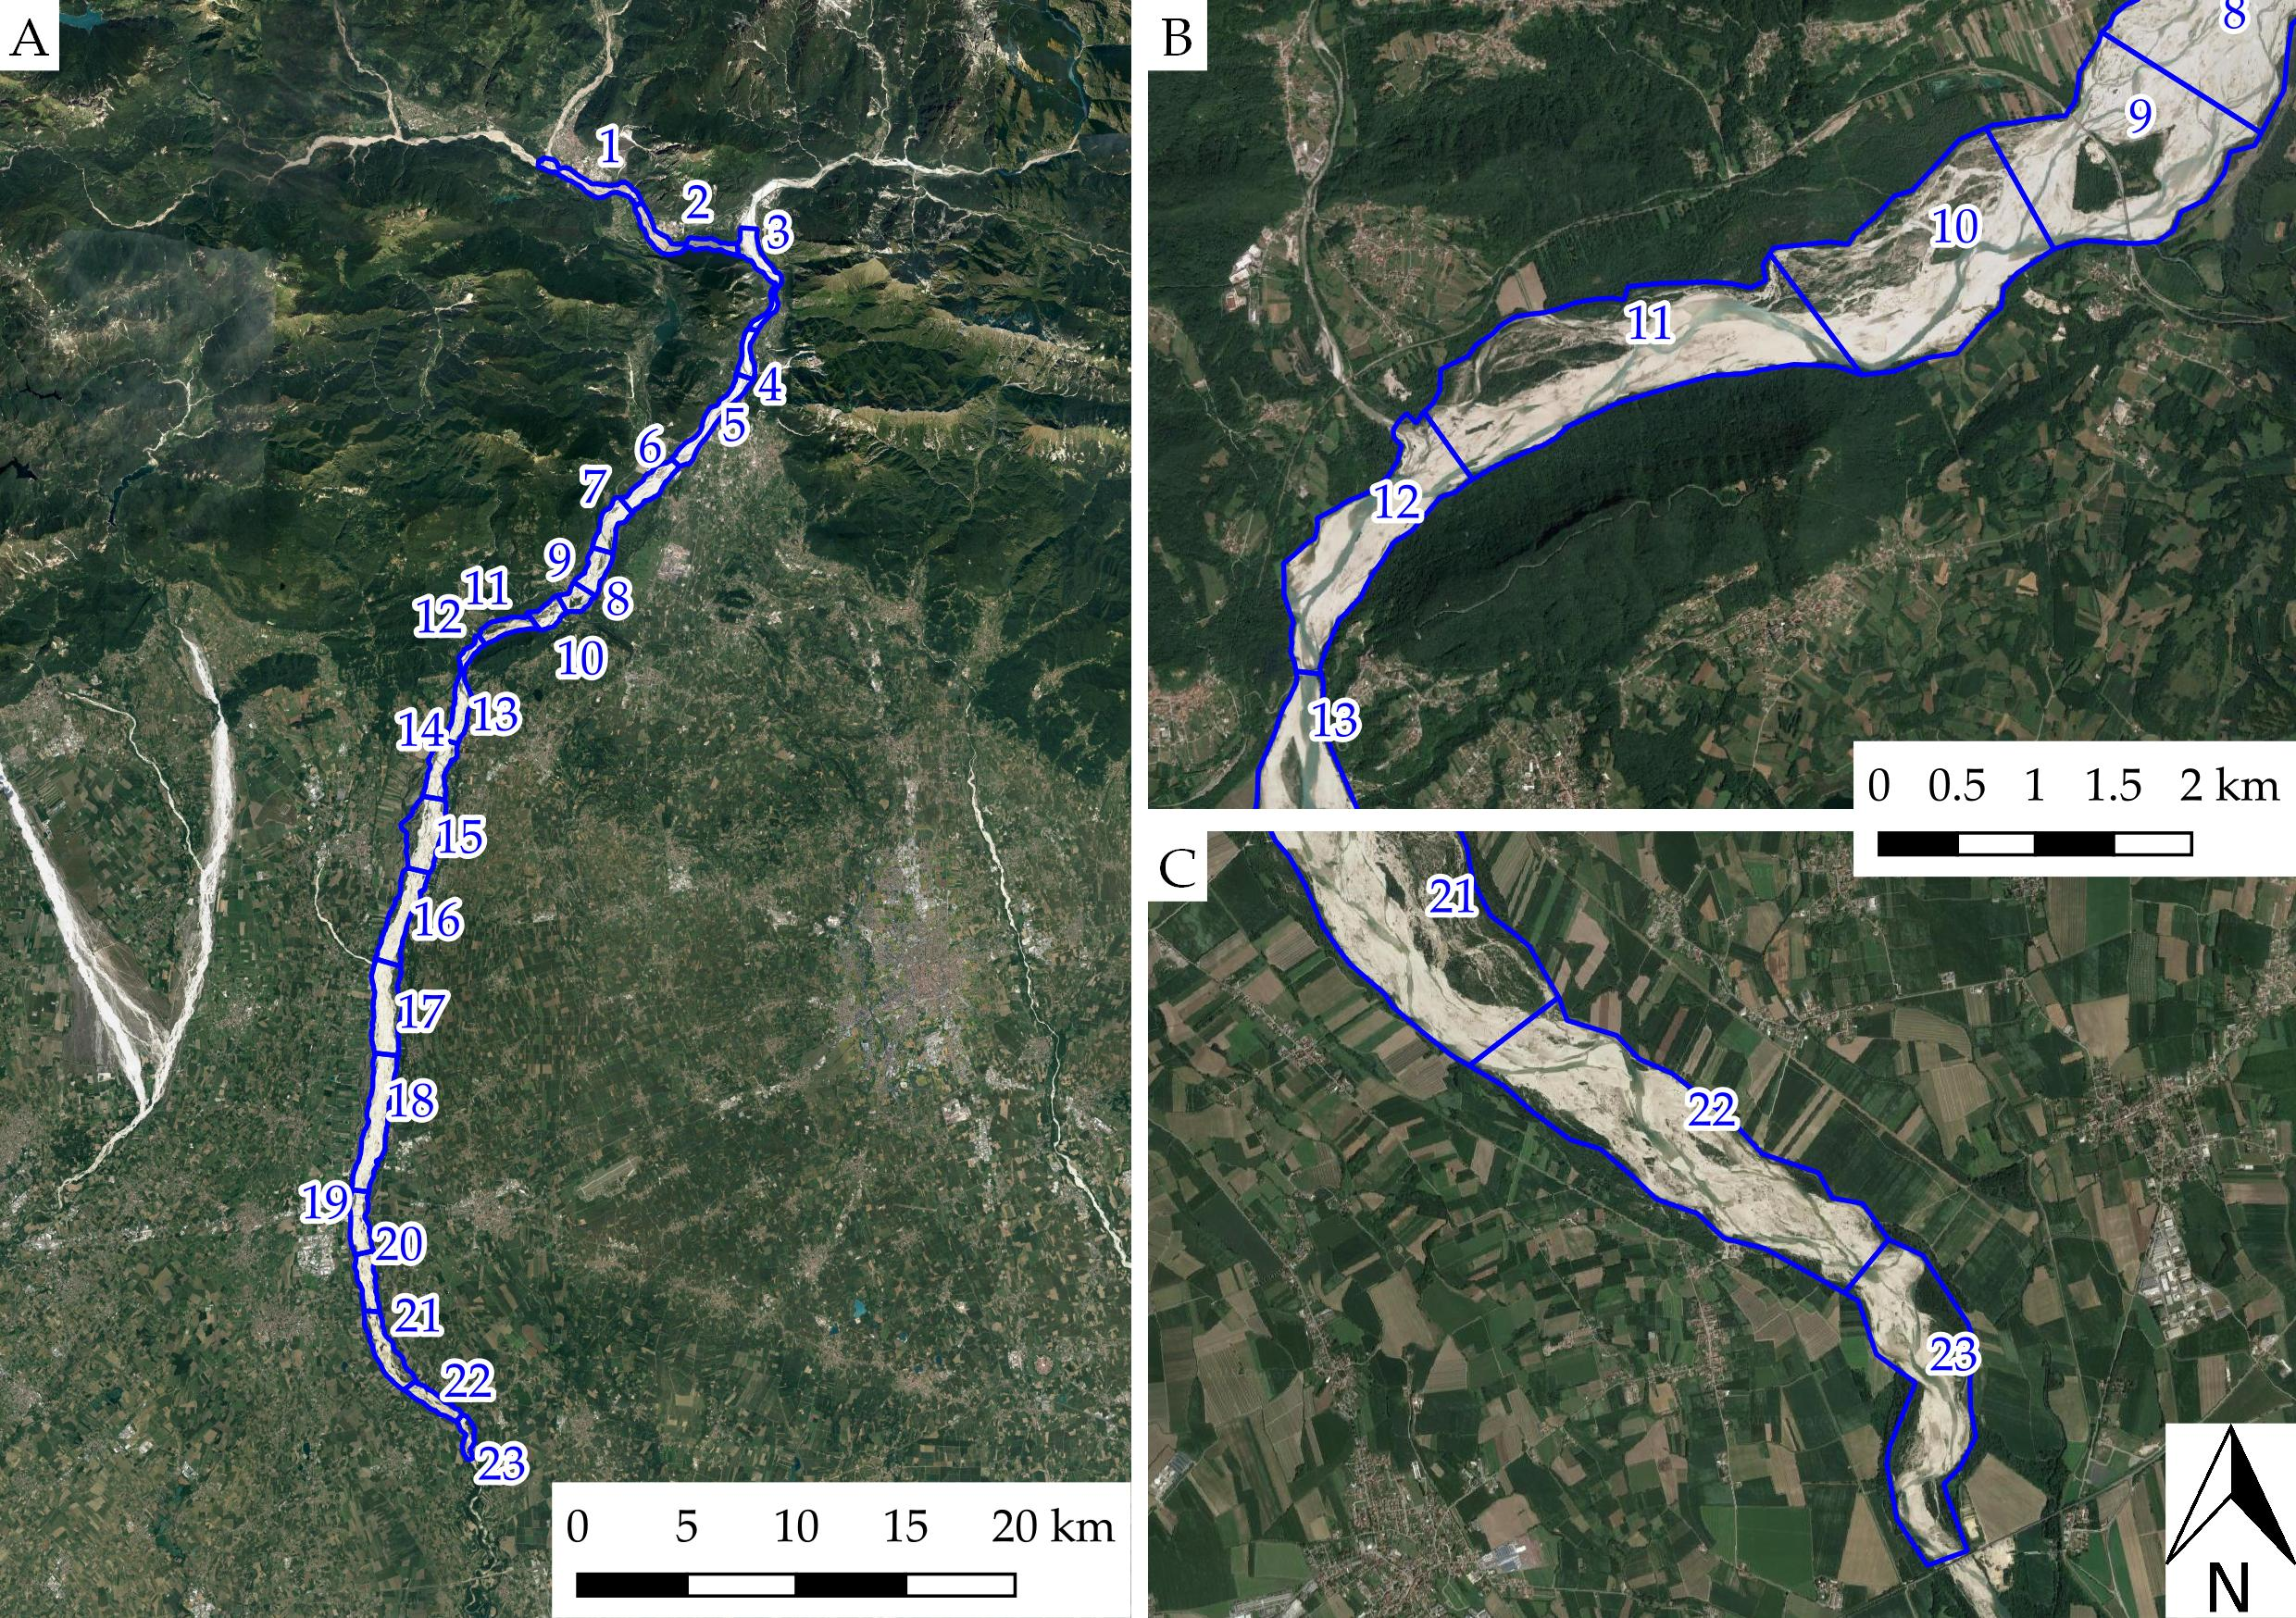
\includegraphics[width=.8\textwidth]{files/tutti_23_tratti.jpeg}
		\caption[immagine con la maschera suddivisa in 23 tratti]{immagine con la maschera suddivisa in 23 tratti; la sezione di monte del tratto~1 corrisponde a Tolmezzo, la sezione di valle del tratto~23 corrisponde al ponte di Madrisio.}
		\label{fig:23-tratti}
	\end{figure}
	%
	%
	\item[isole e \emph{Floodplain}]
	Tramite una procedura semi-automatica e con il supporto di Google Earth, la classe della vegetazione è stata suddivisa in \emph{floodplain} e isole. 
	Tale procedura si basa sul fatto che la maschera computazionale comprende parte della piana alluvionale e che le isole sono completamente circondate dalla ghiaia dell'alveo durante periodi di magra.
	\\
	Successivamente, un controllo visivo del risultato e una correzione manuale di alcune celle hanno permesso sia di distinguere correttamente le isole, sia di evitare che isole molto prossime alla \emph{floodplain} ne fossero considerate parte; la classe delle celle corrette è stata aggiunta alla classificazione.
	%
	%
	\item[Nuvole e nodata] Alcune immagini presentano una lieve copertura nuvolosa che si estende nella maschera; queste zone sono state manualmente delimitate poiché presentano valori NDVI alterati.
	\\
	Altre immagini hanno un'estensione limitata rispetto alla maschera; questo porta ad avere aree prive di dati (\texttt{nodata}).
	\\
	Alla classificazione sono state aggiunte la classe delle nuvole e dei \texttt{nodata}.
	%
	%
	\item[Classificazione finale dei tratti] La \vref{tab:class_tratti} mostra le classi in cui è stato classificato ognuno dei 23~tratti; la %\vref{fig:class_is_fl} ne mostra un esempio.
	%
	\begin{table}[ht]
		\centering
		\begin{tabular}{
			c 
			c
			}
			\toprule
			\textbf{Macroclasse}	&	\textbf{Classe}	\\
			\midrule
			Vegetazione		&	Isola	\\
							&	Floodplain	\\
			Alveo attivo	&	Cella corretta	\\
							&	Ghiaia	\\
							&	Canale	\\
			Altro			&	Nuvola	\\
							&	Nodata	\\
			\bottomrule
		\end{tabular}
		\caption[classificazione dell'area dei tratti]{classificazione finale dell'area di ogni tratto all'interno della maschera computazionale.}
		\label{tab:class_tratti}
	\end{table}
	%
	\begin{figure}[ht]
		\centering
		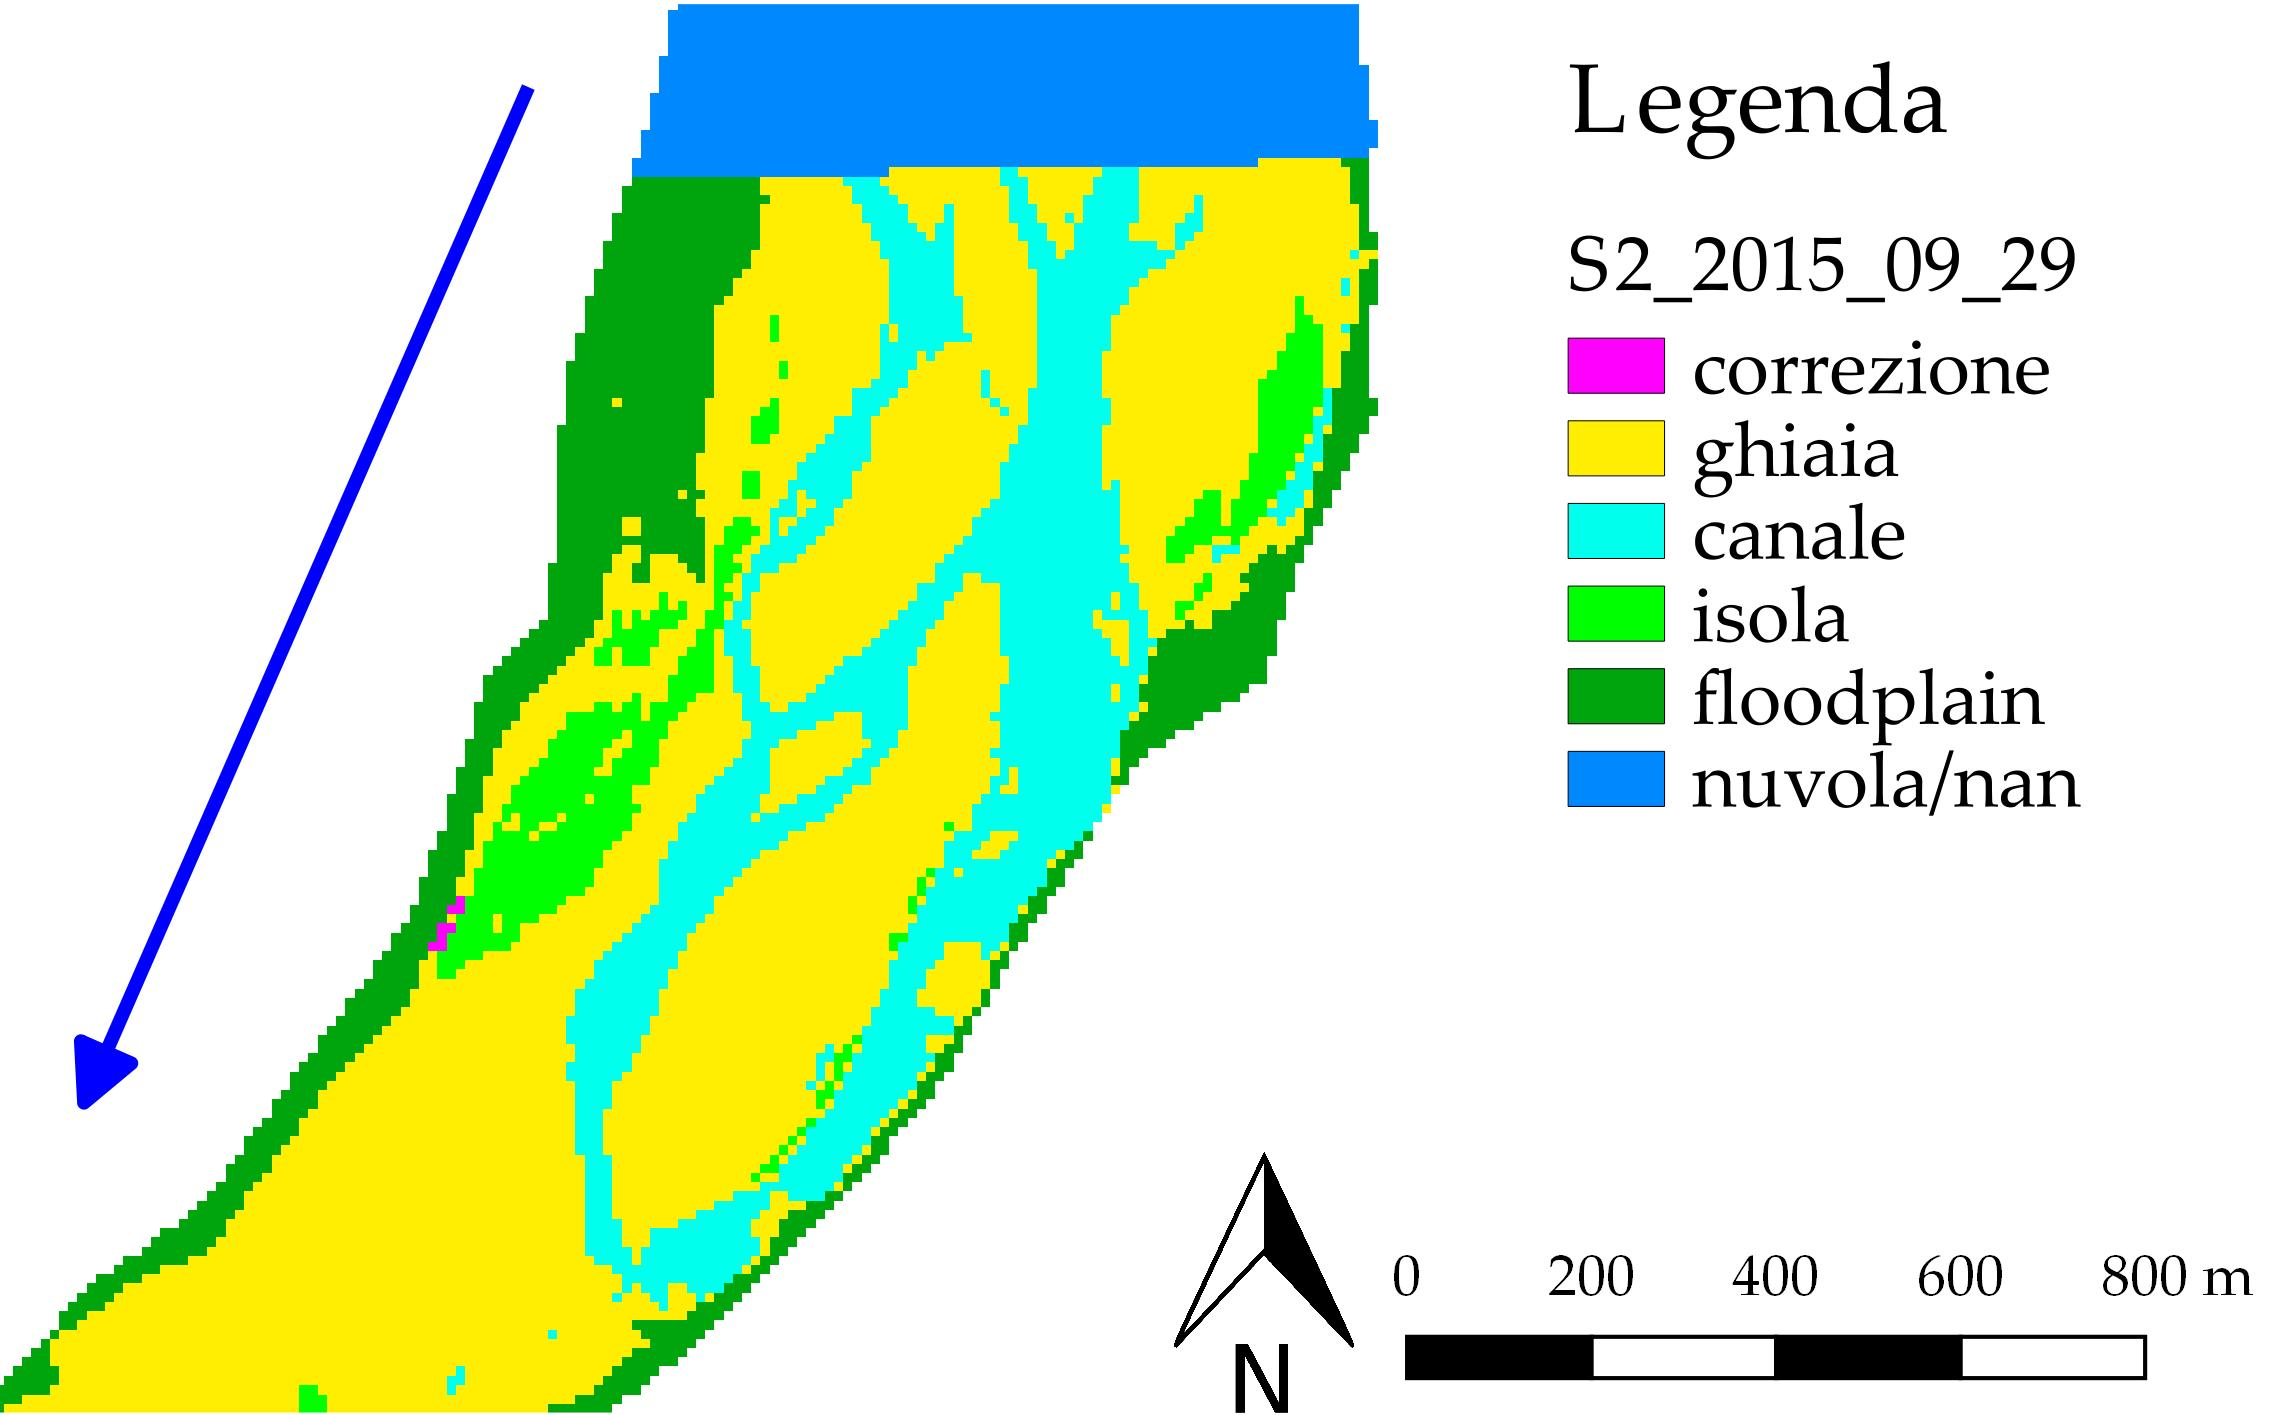
\includegraphics[width=.8\textwidth]{files/esempio_class_is_fl.jpeg}
		\caption[esempio della classificazione dell'area dei tratti]{esempio della classificazione dell'area dei tratti.}
		\label{fig:class_is_fl}
	\end{figure}
	%
	Al fine di validare la precedente procedura di controllo e correzione della distinzione isole - \emph{floodplain}, si è osservato per ogni tratto l'andamento temporale della larghezza media~$B$, esprimibile semplicemente come il rapporto dell'area dell'alveo di ogni tratto (somma dell'alveo attivo e delle isole) per la sua lunghezza seguendo la corrente:
	%
	\begin{equation}
		B = \frac{\text{Area alveo}}{Lunghezza} 
		\quad .
		\label{eq:larghezza_tratto}
	\end{equation}
	% 
	Si è verificato che la larghezza~$B$ rimanesse costante nel tempo, indice di una corretta classificazione tra isole e \emph{floodplain}. 
	La~$B$ non rimane costante solo nel caso di distacco di isole o di fusione di isole nella piana. 
	\\
	La \vref{fig:b-media-7-e-15} mostra l'andamento temporale della~$B$ dei tratti~7 e~15: nel primo tratto, in cui non si osserva alcuna variazione sensibile dell'alveo, la~$B$ oscilla solo di qualche decina di metri; nel secondo si assiste alla progressiva fusione di una grande isola nella \emph{floodplain}, e questo lo si vede proprio nella diminuzione della~$B$. Ciò che conta non è quanto è largo l'alveo, ma quanto cambia la larghezza.
	%
	\begin{figure}
		\centering
		\begin{tikzpicture}
	\begin{axis}[
		width = 0.6\textwidth,
		height = 0.5\textwidth,
		date coordinates in = x,
		xticklabel = {\year},
		xticklabel style = {
			rotate = 80,
			anchor = near xticklabel
		},
		xtick distance = 730,
		enlarge x limits = 0.05,
		enlarge y limits = 0.01,
		%ymax = 3.7,
		%ymin = -0.1,
		%ytick distance = 0.5,
		ylabel = {Larghezza media dell'alveo \si{[\m]}},
		grid = major,
		]
		\addplot+
        	[blue]
        	table [x=data, y=tr_7] {graphics/data/Larghezze_medie_alveo.txt};
        \addlegendentry{Tratto 7}
        
		\addplot+
        	[orange]
        	table [x=data, y=tr_15] {graphics/data/Larghezze_medie_alveo.txt};
        \addlegendentry{Tratto 15}
	\end{axis}
\end{tikzpicture}

		\quad
		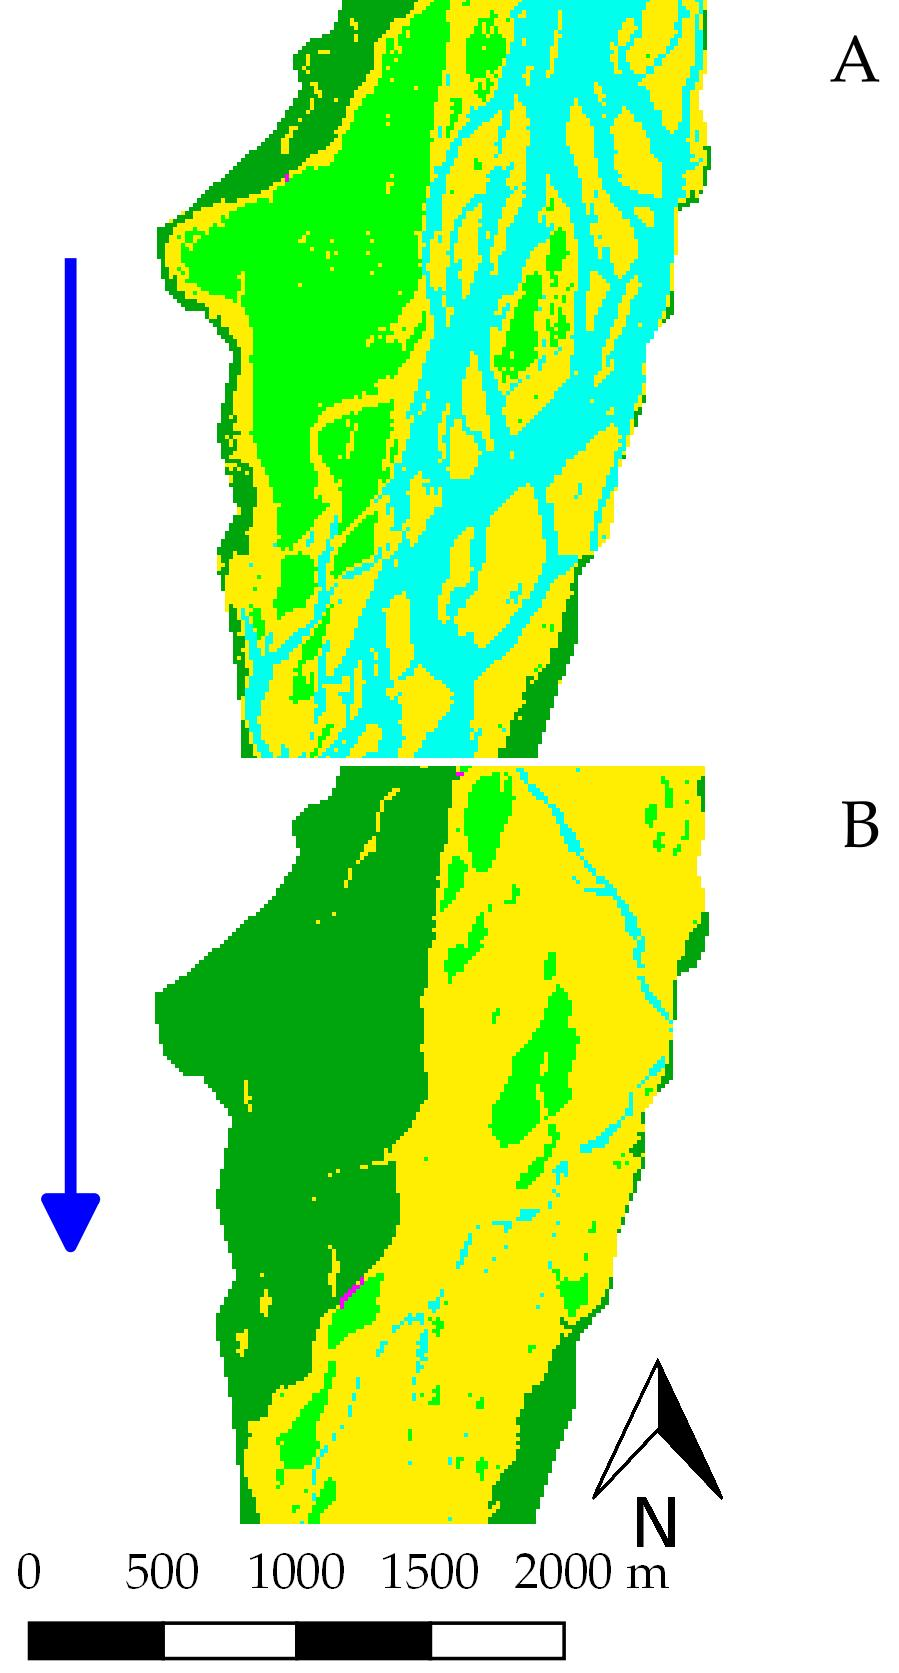
\includegraphics[width=0.3\textwidth]{files/fusione_isola_tr_15.jpeg}
		\caption[andamento temporale di $B$ per i tratti~7 e~15]{a sinistra si vede l'andamento nel tempo della larghezza media dei tratti~7 e~15; la $B$ del tratto~7 oscilla solamente di qualche decina di metri, mentre il tratto~15 riduce improvvisamente la sua $B$ a causa della fusione di una grande isola nella \emph{floodplain}, fenomeno mostrato a destra (A: 2003-11-29, B: 2005-08-30).}
		\label{fig:b-media-7-e-15}
	\end{figure}
	
\end{description}


% tenere questa parte? forse la si può togliere
% e mostrare direttamente i risultati sul cambiamento
Con la riclassificazione delle immagini dell'NDVI rispetto alle soglie proposte è stato possibile ottenere la percentuale di alveo coperta da vegetazione per ogni anno. 
Si ricorda, grazie alla maschera applicata, tale copertura include sia isole vegetate sia la parte di piana alluvionale che nel periodo di studio ha esperito fenomeni di erosione della vegetazione e quindi espansione dell'alveo attivo.
Infine, per le immagini l'alveo parzialmente coperto da nuvole, la maschera è stata estesa per escludere tali zone coperte poiché queste presentano valori di NDVI non corretti.
\\
I risultati sono mostrati nel grafico in \vref{graph:class-sat-veg}.


\begin{figure}[ht]
	\centering
	\begin{tikzpicture}
	\begin{axis}[
		width = \textwidth,
		height = 0.5\textwidth,
		date coordinates in = x,
		date ZERO = 2000-01-01,
		xticklabel = {\year},
		xticklabel style = {
			rotate = 80,
			anchor = near xticklabel
		},
		axis y line* = right,
		ymax = 70,
		%ymin = 0,
		ylabel = {Percentuale di vegetazione},
		grid = none,
		]
		\addplot+
        	[red, mark=+, ultra thick]
        	table [x=data, y=veg] {graphics/data/Class_sat_veg-H2O-ghiaia.txt};
	\end{axis}
	
	\begin{axis}[
		width = \textwidth,
		height = 0.5\textwidth,
		date coordinates in = x,
		date ZERO = 2000-01-01,
		xticklabel = {\year},
		xticklabel style = {
			rotate = 80,
			anchor = near xticklabel
		},
		axis y line* = left,
		axis x line = none,
		enlarge x limits = 0.05,
		enlarge y limits = 0.01,
		ymax = 3.7,
		ymin = 2,
		ylabel = {Livello idrometrico},
		grid = none,
		]
		\addplot+
        	[blue, no markers, ultra thin]
        	table [x=data, y=media-gg] {graphics/data/Dati_Villuzza.csv};
	\end{axis}
\end{tikzpicture}

	\caption[andamento dell'areale della vegetazione nelle isole  e nella floodplain]{andamento dell'areale della vegetazione nelle isole e nella floodplain (in rosso). I dati provengono dalla classificazione delle immagini satellitari (ASTER, Pleiades, Sentinel2 e WorldView2). In blu sono mostrati i livelli idrometrici medi giornalieri superiori a~\SI{2}{\m} registrati alla stazione di Villuzza.}
	\label{graph:class-sat-veg}
\end{figure}


% grafico piene 2m+ - %veg tratti (nuovo file comprensivo di tutti i tratti)



% nuova sezione sul cambiamento della vegetazione


% cambiamento della vegetazione
% spostamento delle immagini che lo necessitano

% età della vegetazione




%----------------------------------------------------------



%**********************************************************
%**********************************************************
\backmatter
\printbibliography

\end{document}
